\documentclass[a4paper]{book}
\usepackage{a4wide}
\usepackage{makeidx}
\usepackage{graphicx}
\usepackage{multicol}
\usepackage{float}
\usepackage{listings}
\usepackage{color}
\usepackage{textcomp}
\usepackage{alltt}
\usepackage{times}
\usepackage{ifpdf}
\ifpdf
\usepackage[pdftex,
            pagebackref=true,
            colorlinks=true,
            linkcolor=blue,
            unicode
           ]{hyperref}
\else
\usepackage[ps2pdf,
            pagebackref=true,
            colorlinks=true,
            linkcolor=blue,
            unicode
           ]{hyperref}
\usepackage{pspicture}
\fi
\usepackage[utf8]{inputenc}
\usepackage{doxygen}
\lstset{language=C++,inputencoding=utf8,basicstyle=\footnotesize,breaklines=true,breakatwhitespace=true,tabsize=8,numbers=left }
\makeindex
\setcounter{tocdepth}{3}
\renewcommand{\footrulewidth}{0.4pt}
\begin{document}
\hypersetup{pageanchor=false}
\begin{titlepage}
\vspace*{7cm}
\begin{center}
{\Large Shopped \\[1ex]\large We have draw functionality now! :) }\\
\vspace*{1cm}
{\large Generated by Doxygen 1.6.1}\\
\vspace*{0.5cm}
{\small Sun Nov 15 20:59:53 2009}\\
\end{center}
\end{titlepage}
\clearemptydoublepage
\pagenumbering{roman}
\tableofcontents
\clearemptydoublepage
\pagenumbering{arabic}
\hypersetup{pageanchor=true}
\chapter{Class Index}
\section{Class Hierarchy}
This inheritance list is sorted roughly, but not completely, alphabetically:\begin{DoxyCompactList}
\item \contentsline{section}{Core.Images.CurrentImage}{\pageref{class_core_1_1_images_1_1_current_image}}{}
\item \contentsline{section}{Core.Interfaces.IFileOperations}{\pageref{interface_core_1_1_interfaces_1_1_i_file_operations}}{}
\begin{DoxyCompactList}
\item \contentsline{section}{Core.FileOperations}{\pageref{class_core_1_1_file_operations}}{}
\end{DoxyCompactList}
\item \contentsline{section}{Core.ImageRotate}{\pageref{class_core_1_1_image_rotate}}{}
\item \contentsline{section}{UI.Properties.Resources}{\pageref{class_u_i_1_1_properties_1_1_resources}}{}
\item \contentsline{section}{UI.RotateDialog}{\pageref{class_u_i_1_1_rotate_dialog}}{}
\item \contentsline{section}{UI.Properties.Settings}{\pageref{class_u_i_1_1_properties_1_1_settings}}{}
\item \contentsline{section}{UI.ShoppedGui}{\pageref{class_u_i_1_1_shopped_gui}}{}
\end{DoxyCompactList}

\chapter{Class Index}
\section{Class List}
Here are the classes, structs, unions and interfaces with brief descriptions:\begin{DoxyCompactList}
\item\contentsline{section}{\hyperlink{class_core_1_1_images_1_1_current_image}{Core::Images::CurrentImage} }{\pageref{class_core_1_1_images_1_1_current_image}}{}
\item\contentsline{section}{\hyperlink{class_core_1_1_file_operations}{Core::FileOperations} }{\pageref{class_core_1_1_file_operations}}{}
\item\contentsline{section}{\hyperlink{interface_core_1_1_interfaces_1_1_i_file_operations}{Core::Interfaces::IFileOperations} }{\pageref{interface_core_1_1_interfaces_1_1_i_file_operations}}{}
\item\contentsline{section}{\hyperlink{class_core_1_1_image_rotate}{Core::ImageRotate} }{\pageref{class_core_1_1_image_rotate}}{}
\item\contentsline{section}{\hyperlink{class_u_i_1_1_resize_dialog}{UI::ResizeDialog} }{\pageref{class_u_i_1_1_resize_dialog}}{}
\item\contentsline{section}{\hyperlink{class_u_i_1_1_properties_1_1_resources}{UI::Properties::Resources} (A strongly-\/typed resource class, for looking up localized strings, etc )}{\pageref{class_u_i_1_1_properties_1_1_resources}}{}
\item\contentsline{section}{\hyperlink{class_u_i_1_1_rotate_dialog}{UI::RotateDialog} }{\pageref{class_u_i_1_1_rotate_dialog}}{}
\item\contentsline{section}{\hyperlink{class_u_i_1_1_properties_1_1_settings}{UI::Properties::Settings} }{\pageref{class_u_i_1_1_properties_1_1_settings}}{}
\item\contentsline{section}{\hyperlink{class_u_i_1_1_shopped_gui}{UI::ShoppedGui} }{\pageref{class_u_i_1_1_shopped_gui}}{}
\item\contentsline{section}{\hyperlink{class_u_i_1_1_zoom_dialog}{UI::ZoomDialog} }{\pageref{class_u_i_1_1_zoom_dialog}}{}
\end{DoxyCompactList}

\chapter{Class Documentation}
\hypertarget{class_core_1_1_manipulators_1_1_brightness}{
\section{Core::Manipulators::Brightness Class Reference}
\label{class_core_1_1_manipulators_1_1_brightness}\index{Core::Manipulators::Brightness@{Core::Manipulators::Brightness}}
}
\subsection*{Public Member Functions}
\begin{DoxyCompactItemize}
\item 
\hyperlink{class_core_1_1_images_1_1_picture_box_image}{PictureBoxImage} \hyperlink{class_core_1_1_manipulators_1_1_brightness_a1949faa9d47db583717627b1fdda80ce}{AdjustBrightness} (\hyperlink{class_core_1_1_images_1_1_picture_box_image}{PictureBoxImage} pictureBoxImage, float brightnessLevel)
\end{DoxyCompactItemize}


\subsection{Member Function Documentation}
\hypertarget{class_core_1_1_manipulators_1_1_brightness_a1949faa9d47db583717627b1fdda80ce}{
\index{Core::Manipulators::Brightness@{Core::Manipulators::Brightness}!AdjustBrightness@{AdjustBrightness}}
\index{AdjustBrightness@{AdjustBrightness}!Core::Manipulators::Brightness@{Core::Manipulators::Brightness}}
\subsubsection[{AdjustBrightness}]{\setlength{\rightskip}{0pt plus 5cm}{\bf PictureBoxImage} Core::Manipulators::Brightness::AdjustBrightness ({\bf PictureBoxImage} {\em pictureBoxImage}, \/  float {\em brightnessLevel})\hspace{0.3cm}{\ttfamily  \mbox{[}inline\mbox{]}}}}
\label{class_core_1_1_manipulators_1_1_brightness_a1949faa9d47db583717627b1fdda80ce}
A filter that will change the brightness of an image.


\begin{DoxyParams}{Parameters}
\item[{\em pictureBoxImage}]The PictureBoxImage object in the current context of Shopped GUI \end{DoxyParams}
\begin{DoxyReturn}{Returns}
A PictureBoxImage object with the appropriate properties set by this method. 
\end{DoxyReturn}


The documentation for this class was generated from the following file:\begin{DoxyCompactItemize}
\item 
C:/Users/Andy/Documents/Visual Studio 2008/Projects/capstone2009/shopped/src/Core/Manipulators/Brightness.cs\end{DoxyCompactItemize}

\hypertarget{class_u_i_1_1_dialogs_1_1_brightness_dialog}{
\section{UI::Dialogs::BrightnessDialog Class Reference}
\label{class_u_i_1_1_dialogs_1_1_brightness_dialog}\index{UI::Dialogs::BrightnessDialog@{UI::Dialogs::BrightnessDialog}}
}
\subsection*{Public Member Functions}
\begin{DoxyCompactItemize}
\item 
\hyperlink{class_u_i_1_1_dialogs_1_1_brightness_dialog_a1d76ea754eeee6083a1b13e1c468b4d4}{BrightnessDialog} ()
\end{DoxyCompactItemize}
\subsection*{Public Attributes}
\begin{DoxyCompactItemize}
\item 
\hypertarget{class_u_i_1_1_dialogs_1_1_brightness_dialog_a70b6bd43eb4bc3c29a67629cc8918c61}{
float {\bfseries BrightnessLevel}}
\label{class_u_i_1_1_dialogs_1_1_brightness_dialog_a70b6bd43eb4bc3c29a67629cc8918c61}

\end{DoxyCompactItemize}
\subsection*{Private Member Functions}
\begin{DoxyCompactItemize}
\item 
void \hyperlink{class_u_i_1_1_dialogs_1_1_brightness_dialog_a62c4999f69f1f50776ee4a674c73ed95}{AcceptButton\_\-Click} (object sender, EventArgs e)
\end{DoxyCompactItemize}


\subsection{Constructor \& Destructor Documentation}
\hypertarget{class_u_i_1_1_dialogs_1_1_brightness_dialog_a1d76ea754eeee6083a1b13e1c468b4d4}{
\index{UI::Dialogs::BrightnessDialog@{UI::Dialogs::BrightnessDialog}!BrightnessDialog@{BrightnessDialog}}
\index{BrightnessDialog@{BrightnessDialog}!UI::Dialogs::BrightnessDialog@{UI::Dialogs::BrightnessDialog}}
\subsubsection[{BrightnessDialog}]{\setlength{\rightskip}{0pt plus 5cm}UI::Dialogs::BrightnessDialog::BrightnessDialog ()\hspace{0.3cm}{\ttfamily  \mbox{[}inline\mbox{]}}}}
\label{class_u_i_1_1_dialogs_1_1_brightness_dialog_a1d76ea754eeee6083a1b13e1c468b4d4}
A constructor for BrignessDialog 

\subsection{Member Function Documentation}
\hypertarget{class_u_i_1_1_dialogs_1_1_brightness_dialog_a62c4999f69f1f50776ee4a674c73ed95}{
\index{UI::Dialogs::BrightnessDialog@{UI::Dialogs::BrightnessDialog}!AcceptButton\_\-Click@{AcceptButton\_\-Click}}
\index{AcceptButton\_\-Click@{AcceptButton\_\-Click}!UI::Dialogs::BrightnessDialog@{UI::Dialogs::BrightnessDialog}}
\subsubsection[{AcceptButton\_\-Click}]{\setlength{\rightskip}{0pt plus 5cm}void UI::Dialogs::BrightnessDialog::AcceptButton\_\-Click (object {\em sender}, \/  EventArgs {\em e})\hspace{0.3cm}{\ttfamily  \mbox{[}inline, private\mbox{]}}}}
\label{class_u_i_1_1_dialogs_1_1_brightness_dialog_a62c4999f69f1f50776ee4a674c73ed95}
Once the user hits the \char`\"{}Accept\char`\"{} button, this grabs the value from the dialog box. 

The documentation for this class was generated from the following file:\begin{DoxyCompactItemize}
\item 
C:/Users/Andy/Documents/Visual Studio 2008/Projects/capstone2009/shopped/src/UI/Dialogs/BrightnessDialog.cs\end{DoxyCompactItemize}

\hypertarget{class_core_1_1_manipulators_1_1_contrast}{
\section{Core::Manipulators::Contrast Class Reference}
\label{class_core_1_1_manipulators_1_1_contrast}\index{Core::Manipulators::Contrast@{Core::Manipulators::Contrast}}
}
\subsection*{Public Member Functions}
\begin{DoxyCompactItemize}
\item 
\hyperlink{class_core_1_1_images_1_1_picture_box_image}{PictureBoxImage} \hyperlink{class_core_1_1_manipulators_1_1_contrast_a8362f6c82ab06aa2ff52d7cb3360b28b}{AdjustContrast} (\hyperlink{class_core_1_1_images_1_1_picture_box_image}{PictureBoxImage} pictureBoxImage, float contrastLevel)
\end{DoxyCompactItemize}
\subsection*{Static Public Member Functions}
\begin{DoxyCompactItemize}
\item 
static T \hyperlink{class_core_1_1_manipulators_1_1_contrast_a4898ce913d2031a4c9fa6fe73eba5c0e}{Clamp$<$ T $>$} (T value, T max, T min)
\end{DoxyCompactItemize}


\subsection{Member Function Documentation}
\hypertarget{class_core_1_1_manipulators_1_1_contrast_a8362f6c82ab06aa2ff52d7cb3360b28b}{
\index{Core::Manipulators::Contrast@{Core::Manipulators::Contrast}!AdjustContrast@{AdjustContrast}}
\index{AdjustContrast@{AdjustContrast}!Core::Manipulators::Contrast@{Core::Manipulators::Contrast}}
\subsubsection[{AdjustContrast}]{\setlength{\rightskip}{0pt plus 5cm}{\bf PictureBoxImage} Core::Manipulators::Contrast::AdjustContrast ({\bf PictureBoxImage} {\em pictureBoxImage}, \/  float {\em contrastLevel})\hspace{0.3cm}{\ttfamily  \mbox{[}inline\mbox{]}}}}
\label{class_core_1_1_manipulators_1_1_contrast_a8362f6c82ab06aa2ff52d7cb3360b28b}
A filter that will change the contrast of an image.


\begin{DoxyParams}{Parameters}
\item[{\em pictureBoxImage}]The PictureBoxImage object in the current context of Shopped GUI \end{DoxyParams}
\begin{DoxyReturn}{Returns}
A PictureBoxImage object with the appropriate properties set by this method. 
\end{DoxyReturn}
\hypertarget{class_core_1_1_manipulators_1_1_contrast_a4898ce913d2031a4c9fa6fe73eba5c0e}{
\index{Core::Manipulators::Contrast@{Core::Manipulators::Contrast}!Clamp$<$ T $>$@{Clamp$<$ T $>$}}
\index{Clamp$<$ T $>$@{Clamp$<$ T $>$}!Core::Manipulators::Contrast@{Core::Manipulators::Contrast}}
\subsubsection[{Clamp$<$ T $>$}]{\setlength{\rightskip}{0pt plus 5cm}static T Core::Manipulators::Contrast::Clamp$<$ T $>$ (T {\em value}, \/  T {\em max}, \/  T {\em min})\hspace{0.3cm}{\ttfamily  \mbox{[}inline, static\mbox{]}}}}
\label{class_core_1_1_manipulators_1_1_contrast_a4898ce913d2031a4c9fa6fe73eba5c0e}
A generic clamp class that make sure the RBG values lie in the specified range. If it is greater than the max value, it is replaced by the max value.


\begin{DoxyParams}{Parameters}
\item[{\em value}]The value being compared \item[{\em max}]The maximum allowed value \item[{\em min}]The minimum allowed value \end{DoxyParams}
\begin{Desc}
\item[Type Constraints]\begin{description}
\item[{\em T} : {\em System.IComparable$<$T$>$}]\end{description}
\end{Desc}


The documentation for this class was generated from the following file:\begin{DoxyCompactItemize}
\item 
C:/Users/Andy/Documents/Visual Studio 2008/Projects/capstone2009/shopped/src/Core/Manipulators/Contrast.cs\end{DoxyCompactItemize}

\hypertarget{class_u_i_1_1_dialogs_1_1_contrast_dialog}{
\section{UI::Dialogs::ContrastDialog Class Reference}
\label{class_u_i_1_1_dialogs_1_1_contrast_dialog}\index{UI::Dialogs::ContrastDialog@{UI::Dialogs::ContrastDialog}}
}
\subsection*{Public Member Functions}
\begin{DoxyCompactItemize}
\item 
\hyperlink{class_u_i_1_1_dialogs_1_1_contrast_dialog_a132eec552bc31b9d0824812157ac314e}{ContrastDialog} ()
\end{DoxyCompactItemize}
\subsection*{Public Attributes}
\begin{DoxyCompactItemize}
\item 
\hypertarget{class_u_i_1_1_dialogs_1_1_contrast_dialog_afb9f579b72aad49311a387e4cf73f573}{
float {\bfseries ContrastLevel}}
\label{class_u_i_1_1_dialogs_1_1_contrast_dialog_afb9f579b72aad49311a387e4cf73f573}

\end{DoxyCompactItemize}
\subsection*{Private Member Functions}
\begin{DoxyCompactItemize}
\item 
void \hyperlink{class_u_i_1_1_dialogs_1_1_contrast_dialog_a09bc379f0949d32c392a26672150246d}{AcceptButton\_\-Click} (object sender, EventArgs e)
\end{DoxyCompactItemize}


\subsection{Constructor \& Destructor Documentation}
\hypertarget{class_u_i_1_1_dialogs_1_1_contrast_dialog_a132eec552bc31b9d0824812157ac314e}{
\index{UI::Dialogs::ContrastDialog@{UI::Dialogs::ContrastDialog}!ContrastDialog@{ContrastDialog}}
\index{ContrastDialog@{ContrastDialog}!UI::Dialogs::ContrastDialog@{UI::Dialogs::ContrastDialog}}
\subsubsection[{ContrastDialog}]{\setlength{\rightskip}{0pt plus 5cm}UI::Dialogs::ContrastDialog::ContrastDialog ()\hspace{0.3cm}{\ttfamily  \mbox{[}inline\mbox{]}}}}
\label{class_u_i_1_1_dialogs_1_1_contrast_dialog_a132eec552bc31b9d0824812157ac314e}
A constructor for \hyperlink{class_u_i_1_1_dialogs_1_1_contrast_dialog}{ContrastDialog} 

\subsection{Member Function Documentation}
\hypertarget{class_u_i_1_1_dialogs_1_1_contrast_dialog_a09bc379f0949d32c392a26672150246d}{
\index{UI::Dialogs::ContrastDialog@{UI::Dialogs::ContrastDialog}!AcceptButton\_\-Click@{AcceptButton\_\-Click}}
\index{AcceptButton\_\-Click@{AcceptButton\_\-Click}!UI::Dialogs::ContrastDialog@{UI::Dialogs::ContrastDialog}}
\subsubsection[{AcceptButton\_\-Click}]{\setlength{\rightskip}{0pt plus 5cm}void UI::Dialogs::ContrastDialog::AcceptButton\_\-Click (object {\em sender}, \/  EventArgs {\em e})\hspace{0.3cm}{\ttfamily  \mbox{[}inline, private\mbox{]}}}}
\label{class_u_i_1_1_dialogs_1_1_contrast_dialog_a09bc379f0949d32c392a26672150246d}
Once the user hits the \char`\"{}Accept\char`\"{} button, this grabs the value from the dialog box. 

The documentation for this class was generated from the following file:\begin{DoxyCompactItemize}
\item 
C:/Users/Andy/Documents/Visual Studio 2008/Projects/capstone2009/shopped/src/UI/Dialogs/ContrastDialog.cs\end{DoxyCompactItemize}

\hypertarget{class_u_i_1_1_dialogs_1_1_drawing_dialog}{
\section{UI::Dialogs::DrawingDialog Class Reference}
\label{class_u_i_1_1_dialogs_1_1_drawing_dialog}\index{UI::Dialogs::DrawingDialog@{UI::Dialogs::DrawingDialog}}
}
\subsection*{Public Member Functions}
\begin{DoxyCompactItemize}
\item 
\hyperlink{class_u_i_1_1_dialogs_1_1_drawing_dialog_ae813ace4331c45a149293a322e6bbbd4}{DrawingDialog} (\hyperlink{class_core_1_1_manipulators_1_1_image_draw}{ImageDraw} imageDraw)
\end{DoxyCompactItemize}
\subsection*{Public Attributes}
\begin{DoxyCompactItemize}
\item 
\hypertarget{class_u_i_1_1_dialogs_1_1_drawing_dialog_aa60de533b81229d1c4edd0b8ce0583f1}{
\hyperlink{class_core_1_1_manipulators_1_1_image_draw}{ImageDraw} {\bfseries ImageDraw}}
\label{class_u_i_1_1_dialogs_1_1_drawing_dialog_aa60de533b81229d1c4edd0b8ce0583f1}

\end{DoxyCompactItemize}
\subsection*{Private Member Functions}
\begin{DoxyCompactItemize}
\item 
void \hyperlink{class_u_i_1_1_dialogs_1_1_drawing_dialog_a14fc47e4971a3fadfcbcf99be9c3eb4e}{lineColorButton\_\-Click} (object sender, EventArgs e)
\item 
void \hyperlink{class_u_i_1_1_dialogs_1_1_drawing_dialog_a4c405e122958325c0f07fd98ccff8bf2}{okButton\_\-Click} (object sender, EventArgs e)
\item 
void \hyperlink{class_u_i_1_1_dialogs_1_1_drawing_dialog_acda4517c3c2401d544727990f18b8ef6}{lineStyleComboBox\_\-SelectedIndexChanged} (object sender, EventArgs e)
\end{DoxyCompactItemize}


\subsection{Detailed Description}
Performs the actions necessary to grab the drawing info from the dialog box and set the ImageDraw properties accordingly.


\begin{DoxyParams}{Parameters}
\item[{\em ImageDraw}]A new instance of ImageDraw class that will contain the new values. \end{DoxyParams}


\subsection{Constructor \& Destructor Documentation}
\hypertarget{class_u_i_1_1_dialogs_1_1_drawing_dialog_ae813ace4331c45a149293a322e6bbbd4}{
\index{UI::Dialogs::DrawingDialog@{UI::Dialogs::DrawingDialog}!DrawingDialog@{DrawingDialog}}
\index{DrawingDialog@{DrawingDialog}!UI::Dialogs::DrawingDialog@{UI::Dialogs::DrawingDialog}}
\subsubsection[{DrawingDialog}]{\setlength{\rightskip}{0pt plus 5cm}UI::Dialogs::DrawingDialog::DrawingDialog ({\bf ImageDraw} {\em imageDraw})\hspace{0.3cm}{\ttfamily  \mbox{[}inline\mbox{]}}}}
\label{class_u_i_1_1_dialogs_1_1_drawing_dialog_ae813ace4331c45a149293a322e6bbbd4}
Constructor that sets the values of the dialog based on the current ImageDraw settings.


\begin{DoxyParams}{Parameters}
\item[{\em imageDraw}]The ImageDraw object that contains the current settings. \end{DoxyParams}


\subsection{Member Function Documentation}
\hypertarget{class_u_i_1_1_dialogs_1_1_drawing_dialog_a14fc47e4971a3fadfcbcf99be9c3eb4e}{
\index{UI::Dialogs::DrawingDialog@{UI::Dialogs::DrawingDialog}!lineColorButton\_\-Click@{lineColorButton\_\-Click}}
\index{lineColorButton\_\-Click@{lineColorButton\_\-Click}!UI::Dialogs::DrawingDialog@{UI::Dialogs::DrawingDialog}}
\subsubsection[{lineColorButton\_\-Click}]{\setlength{\rightskip}{0pt plus 5cm}void UI::Dialogs::DrawingDialog::lineColorButton\_\-Click (object {\em sender}, \/  EventArgs {\em e})\hspace{0.3cm}{\ttfamily  \mbox{[}inline, private\mbox{]}}}}
\label{class_u_i_1_1_dialogs_1_1_drawing_dialog_a14fc47e4971a3fadfcbcf99be9c3eb4e}
Opens up a color dialog for the user to choose a new color for the draw utility. \hypertarget{class_u_i_1_1_dialogs_1_1_drawing_dialog_acda4517c3c2401d544727990f18b8ef6}{
\index{UI::Dialogs::DrawingDialog@{UI::Dialogs::DrawingDialog}!lineStyleComboBox\_\-SelectedIndexChanged@{lineStyleComboBox\_\-SelectedIndexChanged}}
\index{lineStyleComboBox\_\-SelectedIndexChanged@{lineStyleComboBox\_\-SelectedIndexChanged}!UI::Dialogs::DrawingDialog@{UI::Dialogs::DrawingDialog}}
\subsubsection[{lineStyleComboBox\_\-SelectedIndexChanged}]{\setlength{\rightskip}{0pt plus 5cm}void UI::Dialogs::DrawingDialog::lineStyleComboBox\_\-SelectedIndexChanged (object {\em sender}, \/  EventArgs {\em e})\hspace{0.3cm}{\ttfamily  \mbox{[}inline, private\mbox{]}}}}
\label{class_u_i_1_1_dialogs_1_1_drawing_dialog_acda4517c3c2401d544727990f18b8ef6}
Handler for the changing of the selection in the drop-\/down list for the shape of the draw object. \hypertarget{class_u_i_1_1_dialogs_1_1_drawing_dialog_a4c405e122958325c0f07fd98ccff8bf2}{
\index{UI::Dialogs::DrawingDialog@{UI::Dialogs::DrawingDialog}!okButton\_\-Click@{okButton\_\-Click}}
\index{okButton\_\-Click@{okButton\_\-Click}!UI::Dialogs::DrawingDialog@{UI::Dialogs::DrawingDialog}}
\subsubsection[{okButton\_\-Click}]{\setlength{\rightskip}{0pt plus 5cm}void UI::Dialogs::DrawingDialog::okButton\_\-Click (object {\em sender}, \/  EventArgs {\em e})\hspace{0.3cm}{\ttfamily  \mbox{[}inline, private\mbox{]}}}}
\label{class_u_i_1_1_dialogs_1_1_drawing_dialog_a4c405e122958325c0f07fd98ccff8bf2}
The handler for when the OK button is clicked in the dialog. Grabs the value out of the line thickness text box. 

The documentation for this class was generated from the following file:\begin{DoxyCompactItemize}
\item 
C:/Users/Andy/Documents/Visual Studio 2008/Projects/capstone2009/shopped/src/UI/Dialogs/DrawingDialog.cs\end{DoxyCompactItemize}

\hypertarget{class_core_1_1_file_operations}{
\section{Core::FileOperations Class Reference}
\label{class_core_1_1_file_operations}\index{Core::FileOperations@{Core::FileOperations}}
}
Inheritance diagram for Core::FileOperations::\begin{figure}[H]
\begin{center}
\leavevmode
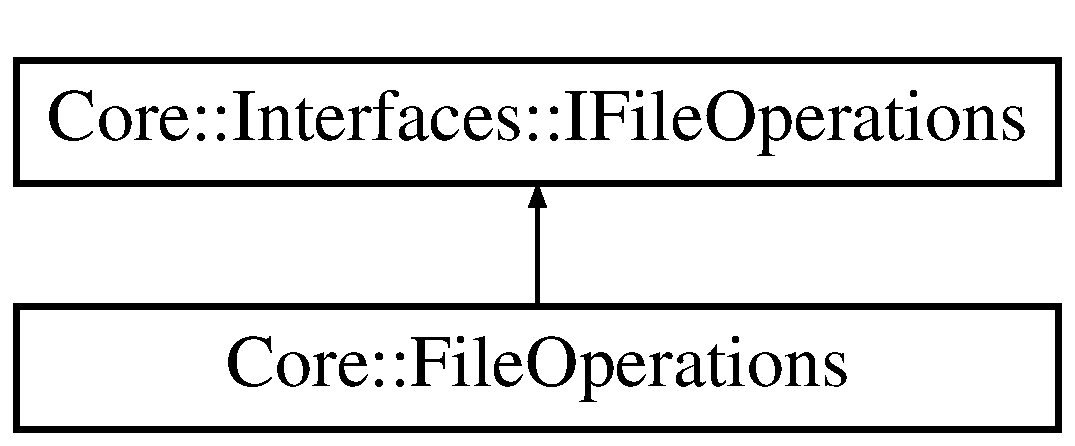
\includegraphics[height=2cm]{class_core_1_1_file_operations}
\end{center}
\end{figure}
\subsection*{Public Member Functions}
\begin{DoxyCompactItemize}
\item 
string \hyperlink{class_core_1_1_file_operations_a23fa84c311fb8051caa8e751d99ef027}{OpenFile} (ref Image imageToOpen)
\item 
void \hyperlink{class_core_1_1_file_operations_a4437acc296a0a32cdf8727ef5a7e94ce}{SaveFile} (Image imageToSave, string fileCurrentlyOpen)
\end{DoxyCompactItemize}


\subsection{Member Function Documentation}
\hypertarget{class_core_1_1_file_operations_a23fa84c311fb8051caa8e751d99ef027}{
\index{Core::FileOperations@{Core::FileOperations}!OpenFile@{OpenFile}}
\index{OpenFile@{OpenFile}!Core::FileOperations@{Core::FileOperations}}
\subsubsection[{OpenFile}]{\setlength{\rightskip}{0pt plus 5cm}string Core::FileOperations::OpenFile (ref Image {\em imageToOpen})\hspace{0.3cm}{\ttfamily  \mbox{[}inline\mbox{]}}}}
\label{class_core_1_1_file_operations_a23fa84c311fb8051caa8e751d99ef027}
Opens a file dialog to select an image, then opens the file inside the Shopped main GUI.


\begin{DoxyParams}{Parameters}
\item[{\em imageToOpen}]This will hold the data of the opened image. \end{DoxyParams}
\begin{DoxyReturn}{Returns}
The absolute path and file name of the opened image. 
\end{DoxyReturn}


Implements \hyperlink{interface_core_1_1_interfaces_1_1_i_file_operations}{Core::Interfaces::IFileOperations}.\hypertarget{class_core_1_1_file_operations_a4437acc296a0a32cdf8727ef5a7e94ce}{
\index{Core::FileOperations@{Core::FileOperations}!SaveFile@{SaveFile}}
\index{SaveFile@{SaveFile}!Core::FileOperations@{Core::FileOperations}}
\subsubsection[{SaveFile}]{\setlength{\rightskip}{0pt plus 5cm}void Core::FileOperations::SaveFile (Image {\em imageToSave}, \/  string {\em fileCurrentlyOpen})\hspace{0.3cm}{\ttfamily  \mbox{[}inline\mbox{]}}}}
\label{class_core_1_1_file_operations_a4437acc296a0a32cdf8727ef5a7e94ce}
Opens a save file dialog to save the image that is open in the Shopped main GUI.


\begin{DoxyParams}{Parameters}
\item[{\em imageToSave}]The image that is currently open in the Shopped main GUI. \item[{\em fileCurrentlyOpen}]The absolute file path to the image that was originally opened in \hyperlink{class_core_1_1_file_operations_a23fa84c311fb8051caa8e751d99ef027}{OpenFile()} \end{DoxyParams}


Implements \hyperlink{interface_core_1_1_interfaces_1_1_i_file_operations}{Core::Interfaces::IFileOperations}.

The documentation for this class was generated from the following file:\begin{DoxyCompactItemize}
\item 
C:/Users/Andy/Documents/Visual Studio 2008/Projects/capstone2009/shopped\_\-iteration1/Core/FileOperations.cs\end{DoxyCompactItemize}

\hypertarget{class_core_1_1_filters_1_1_grayscale}{
\section{Core::Filters::Grayscale Class Reference}
\label{class_core_1_1_filters_1_1_grayscale}\index{Core::Filters::Grayscale@{Core::Filters::Grayscale}}
}
\subsection*{Public Member Functions}
\begin{DoxyCompactItemize}
\item 
\hyperlink{class_core_1_1_images_1_1_picture_box_image}{PictureBoxImage} \hyperlink{class_core_1_1_filters_1_1_grayscale_aed7b431d49987ba71cdf3d232db524b8}{MakeGrayscale} (\hyperlink{class_core_1_1_images_1_1_picture_box_image}{PictureBoxImage} pictureBoxImage)
\end{DoxyCompactItemize}


\subsection{Member Function Documentation}
\hypertarget{class_core_1_1_filters_1_1_grayscale_aed7b431d49987ba71cdf3d232db524b8}{
\index{Core::Filters::Grayscale@{Core::Filters::Grayscale}!MakeGrayscale@{MakeGrayscale}}
\index{MakeGrayscale@{MakeGrayscale}!Core::Filters::Grayscale@{Core::Filters::Grayscale}}
\subsubsection[{MakeGrayscale}]{\setlength{\rightskip}{0pt plus 5cm}{\bf PictureBoxImage} Core::Filters::Grayscale::MakeGrayscale ({\bf PictureBoxImage} {\em pictureBoxImage})\hspace{0.3cm}{\ttfamily  \mbox{[}inline\mbox{]}}}}
\label{class_core_1_1_filters_1_1_grayscale_aed7b431d49987ba71cdf3d232db524b8}
A filter that will make an Image object grayscale.


\begin{DoxyParams}{Parameters}
\item[{\em pictureBoxImage}]The PictureBoxImage object in the current context of Shopped GUI \end{DoxyParams}
\begin{DoxyReturn}{Returns}
A PictureBoxImage object with the appropriate properties set by this method. 
\end{DoxyReturn}


The documentation for this class was generated from the following file:\begin{DoxyCompactItemize}
\item 
C:/Users/Andy/Documents/Visual Studio 2008/Projects/capstone2009/shopped/src/Core/Filters/Grayscale.cs\end{DoxyCompactItemize}

\hypertarget{interface_core_1_1_interfaces_1_1_i_file_operations}{
\section{Core::Interfaces::IFileOperations Interface Reference}
\label{interface_core_1_1_interfaces_1_1_i_file_operations}\index{Core::Interfaces::IFileOperations@{Core::Interfaces::IFileOperations}}
}
Inheritance diagram for Core::Interfaces::IFileOperations::\begin{figure}[H]
\begin{center}
\leavevmode
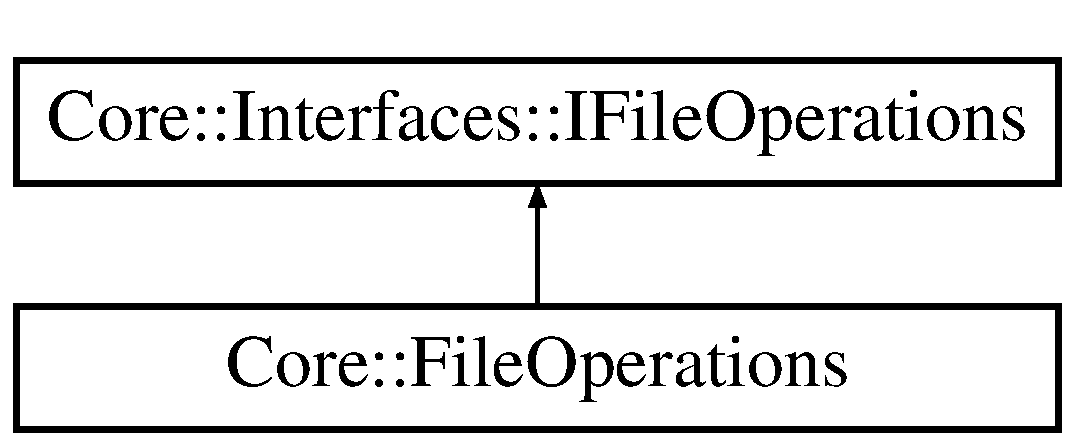
\includegraphics[height=2cm]{interface_core_1_1_interfaces_1_1_i_file_operations}
\end{center}
\end{figure}
\subsection*{Public Member Functions}
\begin{DoxyCompactItemize}
\item 
\hyperlink{class_core_1_1_images_1_1_picture_box_image}{PictureBoxImage} \hyperlink{interface_core_1_1_interfaces_1_1_i_file_operations_a373c3e1cc40a59b65e77cf9551463419}{OpenFile} (\hyperlink{class_core_1_1_images_1_1_picture_box_image}{PictureBoxImage} pictureBoxImage)
\item 
void \hyperlink{interface_core_1_1_interfaces_1_1_i_file_operations_a254301628fd3053115f557626aa71f14}{SaveFile} (\hyperlink{class_core_1_1_images_1_1_picture_box_image}{PictureBoxImage} pictureBoxImage)
\end{DoxyCompactItemize}


\subsection{Detailed Description}
\hyperlink{interface_core_1_1_interfaces_1_1_i_file_operations}{IFileOperations} is an interface to the \hyperlink{class_core_1_1_file_operations}{FileOperations} class. The interface contains two methods, OpenFile and SaveFile. 

\subsection{Member Function Documentation}
\hypertarget{interface_core_1_1_interfaces_1_1_i_file_operations_a373c3e1cc40a59b65e77cf9551463419}{
\index{Core::Interfaces::IFileOperations@{Core::Interfaces::IFileOperations}!OpenFile@{OpenFile}}
\index{OpenFile@{OpenFile}!Core::Interfaces::IFileOperations@{Core::Interfaces::IFileOperations}}
\subsubsection[{OpenFile}]{\setlength{\rightskip}{0pt plus 5cm}{\bf PictureBoxImage} Core::Interfaces::IFileOperations::OpenFile ({\bf PictureBoxImage} {\em pictureBoxImage})}}
\label{interface_core_1_1_interfaces_1_1_i_file_operations_a373c3e1cc40a59b65e77cf9551463419}


Implemented in \hyperlink{class_core_1_1_file_operations_a108130b2bd87d432c0fbbb4f6a42c662}{Core::FileOperations}.\hypertarget{interface_core_1_1_interfaces_1_1_i_file_operations_a254301628fd3053115f557626aa71f14}{
\index{Core::Interfaces::IFileOperations@{Core::Interfaces::IFileOperations}!SaveFile@{SaveFile}}
\index{SaveFile@{SaveFile}!Core::Interfaces::IFileOperations@{Core::Interfaces::IFileOperations}}
\subsubsection[{SaveFile}]{\setlength{\rightskip}{0pt plus 5cm}void Core::Interfaces::IFileOperations::SaveFile ({\bf PictureBoxImage} {\em pictureBoxImage})}}
\label{interface_core_1_1_interfaces_1_1_i_file_operations_a254301628fd3053115f557626aa71f14}


Implemented in \hyperlink{class_core_1_1_file_operations_a0fc5427e96d79e70c6409ec22e70abba}{Core::FileOperations}.

The documentation for this interface was generated from the following file:\begin{DoxyCompactItemize}
\item 
C:/Users/Andy/Documents/Visual Studio 2008/Projects/capstone2009/shopped/Core/Interfaces/\hyperlink{_i_file_operations_8cs}{IFileOperations.cs}\end{DoxyCompactItemize}

\hypertarget{class_core_1_1_manipulators_1_1_image_draw}{
\section{Core::Manipulators::ImageDraw Class Reference}
\label{class_core_1_1_manipulators_1_1_image_draw}\index{Core::Manipulators::ImageDraw@{Core::Manipulators::ImageDraw}}
}
\subsection*{Public Member Functions}
\begin{DoxyCompactItemize}
\item 
\hyperlink{class_core_1_1_manipulators_1_1_image_draw_aab2c1c927b836badfc16cc026a1d0fa5}{ImageDraw} ()
\end{DoxyCompactItemize}
\subsection*{Properties}
\begin{DoxyCompactItemize}
\item 
\hypertarget{class_core_1_1_manipulators_1_1_image_draw_a6e8f48dc18140991e9cf745c80cf6bfe}{
Color {\bfseries LineColor}\hspace{0.3cm}{\ttfamily  \mbox{[}get, set\mbox{]}}}
\label{class_core_1_1_manipulators_1_1_image_draw_a6e8f48dc18140991e9cf745c80cf6bfe}

\item 
\hypertarget{class_core_1_1_manipulators_1_1_image_draw_ae79b1ba4786f10ee7f4d823a78fa26e0}{
int {\bfseries LineThickness}\hspace{0.3cm}{\ttfamily  \mbox{[}get, set\mbox{]}}}
\label{class_core_1_1_manipulators_1_1_image_draw_ae79b1ba4786f10ee7f4d823a78fa26e0}

\item 
\hypertarget{class_core_1_1_manipulators_1_1_image_draw_ab4e8cd78c5cfc30b7d24982107dba4ce}{
string {\bfseries CurrentLineShape}\hspace{0.3cm}{\ttfamily  \mbox{[}get, set\mbox{]}}}
\label{class_core_1_1_manipulators_1_1_image_draw_ab4e8cd78c5cfc30b7d24982107dba4ce}

\item 
\hypertarget{class_core_1_1_manipulators_1_1_image_draw_ad4134232b69f51f9c42755c31207eb45}{
bool {\bfseries Enabled}\hspace{0.3cm}{\ttfamily  \mbox{[}get, set\mbox{]}}}
\label{class_core_1_1_manipulators_1_1_image_draw_ad4134232b69f51f9c42755c31207eb45}

\item 
\hypertarget{class_core_1_1_manipulators_1_1_image_draw_a34171ddf4949ad93bb1466cbe01c5fc7}{
List$<$ string $>$ {\bfseries \_\-lineShapeTypes}\hspace{0.3cm}{\ttfamily  \mbox{[}get, set\mbox{]}}}
\label{class_core_1_1_manipulators_1_1_image_draw_a34171ddf4949ad93bb1466cbe01c5fc7}

\item 
\hypertarget{class_core_1_1_manipulators_1_1_image_draw_a714f8491f101421cec352df654b1d60d}{
List$<$ string $>$ {\bfseries LineShapeTypes}\hspace{0.3cm}{\ttfamily  \mbox{[}get\mbox{]}}}
\label{class_core_1_1_manipulators_1_1_image_draw_a714f8491f101421cec352df654b1d60d}

\end{DoxyCompactItemize}
\subsection*{Private Attributes}
\begin{DoxyCompactItemize}
\item 
\hypertarget{class_core_1_1_manipulators_1_1_image_draw_a9e30e83453c33ee0ac78e088eba006c9}{
{\bfseries Square}}
\label{class_core_1_1_manipulators_1_1_image_draw_a9e30e83453c33ee0ac78e088eba006c9}

\end{DoxyCompactItemize}


\subsection{Detailed Description}
Handles all the drawing functionality.


\begin{DoxyParams}{Parameters}
\item[{\em LineColor}]The color of the line to be drawn. \item[{\em LineThickness}]How wide the line to be drawn will be. \item[{\em LineShape}]The shape of the line (i.e. rounded, square, etc.) \item[{\em Enabled}]Holds whether or not the drawing functionality is enabled. \item[{\em \_\-lineShapeTypes}]The private backing field for LineShapeTypes (can be set). \item[{\em LineShapeTypes}]The public-\/facing list of possible line shapes (read-\/only). \end{DoxyParams}


\subsection{Constructor \& Destructor Documentation}
\hypertarget{class_core_1_1_manipulators_1_1_image_draw_aab2c1c927b836badfc16cc026a1d0fa5}{
\index{Core::Manipulators::ImageDraw@{Core::Manipulators::ImageDraw}!ImageDraw@{ImageDraw}}
\index{ImageDraw@{ImageDraw}!Core::Manipulators::ImageDraw@{Core::Manipulators::ImageDraw}}
\subsubsection[{ImageDraw}]{\setlength{\rightskip}{0pt plus 5cm}Core::Manipulators::ImageDraw::ImageDraw ()\hspace{0.3cm}{\ttfamily  \mbox{[}inline\mbox{]}}}}
\label{class_core_1_1_manipulators_1_1_image_draw_aab2c1c927b836badfc16cc026a1d0fa5}
Default constructor that uses default values. 

The documentation for this class was generated from the following file:\begin{DoxyCompactItemize}
\item 
C:/Users/Andy/Documents/Visual Studio 2008/Projects/capstone2009/shopped/src/Core/Manipulators/ImageDraw.cs\end{DoxyCompactItemize}

\hypertarget{class_core_1_1_image_history}{
\section{Core::ImageHistory Class Reference}
\label{class_core_1_1_image_history}\index{Core::ImageHistory@{Core::ImageHistory}}
}
\subsection*{Public Member Functions}
\begin{DoxyCompactItemize}
\item 
void \hyperlink{class_core_1_1_image_history_a6631d7fefea3a1a28fc6dcdf887daf37}{AddImageToImageHistory} (Image image, string operation)
\item 
Image \hyperlink{class_core_1_1_image_history_ade2a92df5f5525b0e3951b45b2f3434e}{Undo} ()
\item 
Image \hyperlink{class_core_1_1_image_history_afc601ae64181e745d9d94f4b16633a90}{Redo} ()
\item 
int \hyperlink{class_core_1_1_image_history_ae26bcfeed34a733dd372896a86bbc3d4}{GetNumberOfImagesInHistory} ()
\item 
int \hyperlink{class_core_1_1_image_history_a421e672ff9f20e10a03bf989cff4442e}{GetCurrentRevision} ()
\end{DoxyCompactItemize}
\subsection*{Public Attributes}
\begin{DoxyCompactItemize}
\item 
\hypertarget{class_core_1_1_image_history_abb81d12e0bcf3f1f0e79c797f38cc6f2}{
List$<$ \hyperlink{class_core_1_1_image_history_item}{ImageHistoryItem} $>$ {\bfseries ImageRevisions}}
\label{class_core_1_1_image_history_abb81d12e0bcf3f1f0e79c797f38cc6f2}

\end{DoxyCompactItemize}
\subsection*{Private Attributes}
\begin{DoxyCompactItemize}
\item 
\hypertarget{class_core_1_1_image_history_a1a695f64608fc10b95bce32634092f3c}{
int {\bfseries CurrentRevision}}
\label{class_core_1_1_image_history_a1a695f64608fc10b95bce32634092f3c}

\end{DoxyCompactItemize}


\subsection{Detailed Description}
Manages the list of ImageHistoryItems (to do undo and redo) as well as carry out the undo and redo operations. 
\begin{DoxyParams}{Parameters}
\item[{\em ImageRevisions}]A list of \hyperlink{class_core_1_1_image_history_item}{ImageHistoryItem} objects (which contain an Image object and a string detailing the operation). \end{DoxyParams}


\subsection{Member Function Documentation}
\hypertarget{class_core_1_1_image_history_a6631d7fefea3a1a28fc6dcdf887daf37}{
\index{Core::ImageHistory@{Core::ImageHistory}!AddImageToImageHistory@{AddImageToImageHistory}}
\index{AddImageToImageHistory@{AddImageToImageHistory}!Core::ImageHistory@{Core::ImageHistory}}
\subsubsection[{AddImageToImageHistory}]{\setlength{\rightskip}{0pt plus 5cm}void Core::ImageHistory::AddImageToImageHistory (Image {\em image}, \/  string {\em operation})\hspace{0.3cm}{\ttfamily  \mbox{[}inline\mbox{]}}}}
\label{class_core_1_1_image_history_a6631d7fefea3a1a28fc6dcdf887daf37}
Appends the Image object and string passed in to the end of the ImageRevisions list. 
\begin{DoxyParams}{Parameters}
\item[{\em image}]The image to add to the list \item[{\em operation}]A string detailing what operation was just performed \end{DoxyParams}
\hypertarget{class_core_1_1_image_history_a421e672ff9f20e10a03bf989cff4442e}{
\index{Core::ImageHistory@{Core::ImageHistory}!GetCurrentRevision@{GetCurrentRevision}}
\index{GetCurrentRevision@{GetCurrentRevision}!Core::ImageHistory@{Core::ImageHistory}}
\subsubsection[{GetCurrentRevision}]{\setlength{\rightskip}{0pt plus 5cm}int Core::ImageHistory::GetCurrentRevision ()\hspace{0.3cm}{\ttfamily  \mbox{[}inline\mbox{]}}}}
\label{class_core_1_1_image_history_a421e672ff9f20e10a03bf989cff4442e}
Returns the value of the iterator (essentially where we are in the ImageRevisions list). \begin{DoxyReturn}{Returns}
CurrentRevision The value of the iterator for the list. 
\end{DoxyReturn}
\hypertarget{class_core_1_1_image_history_ae26bcfeed34a733dd372896a86bbc3d4}{
\index{Core::ImageHistory@{Core::ImageHistory}!GetNumberOfImagesInHistory@{GetNumberOfImagesInHistory}}
\index{GetNumberOfImagesInHistory@{GetNumberOfImagesInHistory}!Core::ImageHistory@{Core::ImageHistory}}
\subsubsection[{GetNumberOfImagesInHistory}]{\setlength{\rightskip}{0pt plus 5cm}int Core::ImageHistory::GetNumberOfImagesInHistory ()\hspace{0.3cm}{\ttfamily  \mbox{[}inline\mbox{]}}}}
\label{class_core_1_1_image_history_ae26bcfeed34a733dd372896a86bbc3d4}
Returns the number of \hyperlink{class_core_1_1_image_history_item}{ImageHistoryItem} objects on the ImageRevisions list. \begin{DoxyReturn}{Returns}
ImageRevisions.Count() The current number of items in the list. 
\end{DoxyReturn}
\hypertarget{class_core_1_1_image_history_afc601ae64181e745d9d94f4b16633a90}{
\index{Core::ImageHistory@{Core::ImageHistory}!Redo@{Redo}}
\index{Redo@{Redo}!Core::ImageHistory@{Core::ImageHistory}}
\subsubsection[{Redo}]{\setlength{\rightskip}{0pt plus 5cm}Image Core::ImageHistory::Redo ()\hspace{0.3cm}{\ttfamily  \mbox{[}inline\mbox{]}}}}
\label{class_core_1_1_image_history_afc601ae64181e745d9d94f4b16633a90}
Attempts a redo operation by checking if an object exists after the CurrentRevision iterator, then returning that \hyperlink{class_core_1_1_image_history_item}{ImageHistoryItem} node if it does exist. \hypertarget{class_core_1_1_image_history_ade2a92df5f5525b0e3951b45b2f3434e}{
\index{Core::ImageHistory@{Core::ImageHistory}!Undo@{Undo}}
\index{Undo@{Undo}!Core::ImageHistory@{Core::ImageHistory}}
\subsubsection[{Undo}]{\setlength{\rightskip}{0pt plus 5cm}Image Core::ImageHistory::Undo ()\hspace{0.3cm}{\ttfamily  \mbox{[}inline\mbox{]}}}}
\label{class_core_1_1_image_history_ade2a92df5f5525b0e3951b45b2f3434e}
Attempts an undo operation by checking if an object exists before the CurrentRevision iterator, then returning that \hyperlink{class_core_1_1_image_history_item}{ImageHistoryItem} node if it does exist. 

The documentation for this class was generated from the following file:\begin{DoxyCompactItemize}
\item 
C:/Users/Andy/Documents/Visual Studio 2008/Projects/capstone2009/shopped/Core/ImageHistory.cs\end{DoxyCompactItemize}

\hypertarget{class_core_1_1_image_history_item}{
\section{Core::ImageHistoryItem Class Reference}
\label{class_core_1_1_image_history_item}\index{Core::ImageHistoryItem@{Core::ImageHistoryItem}}
}
\subsection*{Properties}
\begin{DoxyCompactItemize}
\item 
\hypertarget{class_core_1_1_image_history_item_af5221965c5ea168e8ce2b248783daa23}{
Image {\bfseries Image}\hspace{0.3cm}{\ttfamily  \mbox{[}get, set\mbox{]}}}
\label{class_core_1_1_image_history_item_af5221965c5ea168e8ce2b248783daa23}

\item 
\hypertarget{class_core_1_1_image_history_item_aa0775d357dd30dafbc2de674b9bcba2b}{
string {\bfseries OperationPerformed}\hspace{0.3cm}{\ttfamily  \mbox{[}get, set\mbox{]}}}
\label{class_core_1_1_image_history_item_aa0775d357dd30dafbc2de674b9bcba2b}

\end{DoxyCompactItemize}


\subsection{Detailed Description}
A simple class that contains an Image object and a string that details the operation performed. 

The documentation for this class was generated from the following file:\begin{DoxyCompactItemize}
\item 
C:/Users/Andy/Documents/Visual Studio 2008/Projects/capstone2009/shopped/Core/ImageHistoryItem.cs\end{DoxyCompactItemize}

\hypertarget{class_tests_1_1_image_history_tester}{
\section{Tests::ImageHistoryTester Class Reference}
\label{class_tests_1_1_image_history_tester}\index{Tests::ImageHistoryTester@{Tests::ImageHistoryTester}}
}
\subsection*{Public Member Functions}
\begin{DoxyCompactItemize}
\item 
\hypertarget{class_tests_1_1_image_history_tester_a83053bb3fba36789ee01460efb9240db}{
void {\bfseries Initialize} ()}
\label{class_tests_1_1_image_history_tester_a83053bb3fba36789ee01460efb9240db}

\item 
\hypertarget{class_tests_1_1_image_history_tester_a26c332961aaa53a5e6df4a8517c81fe6}{
void {\bfseries TearDown} ()}
\label{class_tests_1_1_image_history_tester_a26c332961aaa53a5e6df4a8517c81fe6}

\item 
\hypertarget{class_tests_1_1_image_history_tester_af32c9200363754ffa1fe4b213defb729}{
void {\bfseries CanCreate} ()}
\label{class_tests_1_1_image_history_tester_af32c9200363754ffa1fe4b213defb729}

\item 
\hypertarget{class_tests_1_1_image_history_tester_aa8e0b1ffb021bf9fe281f3705c2738fb}{
void {\bfseries ImageHistoryWithNoImagesIsEmpty} ()}
\label{class_tests_1_1_image_history_tester_aa8e0b1ffb021bf9fe281f3705c2738fb}

\item 
\hypertarget{class_tests_1_1_image_history_tester_ad030fbf52d1e3e6292068fcb0acb88a2}{
void {\bfseries CanAddImageToImageHistory} ()}
\label{class_tests_1_1_image_history_tester_ad030fbf52d1e3e6292068fcb0acb88a2}

\item 
\hypertarget{class_tests_1_1_image_history_tester_a54778f924cc0681ec034c8ea78c7b500}{
void {\bfseries DescriptionGivenToImageHistoryItemIsSetProperly} ()}
\label{class_tests_1_1_image_history_tester_a54778f924cc0681ec034c8ea78c7b500}

\item 
\hypertarget{class_tests_1_1_image_history_tester_a1cd8f49636ad6d34f5b43da9e44c2862}{
void {\bfseries ImageAddedToImageHistoryIsIdenticalToPictureBoxImage} ()}
\label{class_tests_1_1_image_history_tester_a1cd8f49636ad6d34f5b43da9e44c2862}

\item 
\hypertarget{class_tests_1_1_image_history_tester_ab1d89551807ccb29940f83b6c8dcbd40}{
void {\bfseries ImageReturnedByImageHistoryUndoIsIdenticalToOriginal} ()}
\label{class_tests_1_1_image_history_tester_ab1d89551807ccb29940f83b6c8dcbd40}

\item 
\hypertarget{class_tests_1_1_image_history_tester_acaa3c95172e90f5804e31038db2a5bd1}{
void {\bfseries ImageReturnedByImageHistoryUndoThenRedoIsIdenticalToCurrent} ()}
\label{class_tests_1_1_image_history_tester_acaa3c95172e90f5804e31038db2a5bd1}

\item 
\hypertarget{class_tests_1_1_image_history_tester_a35c605d185b3e15d6fc020acb32bf251}{
void {\bfseries GetCurrentRevisionIsNegativeOneOnEmptyImageHistory} ()}
\label{class_tests_1_1_image_history_tester_a35c605d185b3e15d6fc020acb32bf251}

\item 
\hypertarget{class_tests_1_1_image_history_tester_a3b9e48ca23c2f54e07672a71bb9f9e02}{
void {\bfseries GetCurrentRevisionIsZeroAtFirstImageAdded} ()}
\label{class_tests_1_1_image_history_tester_a3b9e48ca23c2f54e07672a71bb9f9e02}

\item 
\hypertarget{class_tests_1_1_image_history_tester_a56a464cd581b73dd07ed5c31db810bae}{
void {\bfseries GetCurrentRevisionIsZeroAfterUndoThenRedo} ()}
\label{class_tests_1_1_image_history_tester_a56a464cd581b73dd07ed5c31db810bae}

\item 
\hypertarget{class_tests_1_1_image_history_tester_a623a6a1617851807780b09d50900fb4c}{
void {\bfseries UndoIsNotPossibleOnEmptyImageHistory} ()}
\label{class_tests_1_1_image_history_tester_a623a6a1617851807780b09d50900fb4c}

\item 
\hypertarget{class_tests_1_1_image_history_tester_a942cf087b58871b937e0f4e4bbbdf0e8}{
void {\bfseries UndoIsPossibleOnImageHistoryWithTwoImagesInHistory} ()}
\label{class_tests_1_1_image_history_tester_a942cf087b58871b937e0f4e4bbbdf0e8}

\item 
\hypertarget{class_tests_1_1_image_history_tester_a849a816b185c0ca81d95c6410c82c970}{
void {\bfseries UndoIsNotPossibleOnImageHistoryWhenIteratorAtLowerBound} ()}
\label{class_tests_1_1_image_history_tester_a849a816b185c0ca81d95c6410c82c970}

\item 
\hypertarget{class_tests_1_1_image_history_tester_a0cdf37b5e3e53ad4772e5516ce38109d}{
void {\bfseries RedoIsNotPossibleOnEmptyImageHistory} ()}
\label{class_tests_1_1_image_history_tester_a0cdf37b5e3e53ad4772e5516ce38109d}

\item 
\hypertarget{class_tests_1_1_image_history_tester_a980859bd655b762088f506f8e846dba9}{
void {\bfseries RedoIsPossibleOnImageHistoryWhenIteratorIsBeforeLastImageInHistory} ()}
\label{class_tests_1_1_image_history_tester_a980859bd655b762088f506f8e846dba9}

\item 
\hypertarget{class_tests_1_1_image_history_tester_abfe02273482ef2bb696eb14d4678ab6c}{
void {\bfseries RedoIsNotPossibleOnImageHistoryWhenIteratorAtRightBound} ()}
\label{class_tests_1_1_image_history_tester_abfe02273482ef2bb696eb14d4678ab6c}

\item 
\hypertarget{class_tests_1_1_image_history_tester_adbca01bd1a1bd7569c33278d55a4b4be}{
void {\bfseries OperationPerformedOnMiddleOfImageHistoryListRemovesImagesAfter} ()}
\label{class_tests_1_1_image_history_tester_adbca01bd1a1bd7569c33278d55a4b4be}

\end{DoxyCompactItemize}
\subsection*{Private Attributes}
\begin{DoxyCompactItemize}
\item 
\hypertarget{class_tests_1_1_image_history_tester_a223c27d8efd1e95d54478eccd9483e06}{
\hyperlink{class_core_1_1_image_history}{ImageHistory} {\bfseries \_\-imageHistory}}
\label{class_tests_1_1_image_history_tester_a223c27d8efd1e95d54478eccd9483e06}

\end{DoxyCompactItemize}


The documentation for this class was generated from the following file:\begin{DoxyCompactItemize}
\item 
C:/Users/Andy/Documents/Visual Studio 2008/Projects/capstone2009/shopped/src/Tests/ImageHistoryTester.cs\end{DoxyCompactItemize}

\hypertarget{class_core_1_1_manipulators_1_1_image_resize}{
\section{Core::Manipulators::ImageResize Class Reference}
\label{class_core_1_1_manipulators_1_1_image_resize}\index{Core::Manipulators::ImageResize@{Core::Manipulators::ImageResize}}
}
\subsection*{Public Member Functions}
\begin{DoxyCompactItemize}
\item 
\hyperlink{class_core_1_1_images_1_1_picture_box_image}{PictureBoxImage} \hyperlink{class_core_1_1_manipulators_1_1_image_resize_a5e36f234fa006a6ce9de380e8fe32798}{ResizeImage} (\hyperlink{class_core_1_1_images_1_1_picture_box_image}{PictureBoxImage} pictureBoxImage, float resize)
\end{DoxyCompactItemize}
\subsection*{Private Attributes}
\begin{DoxyCompactItemize}
\item 
\hypertarget{class_core_1_1_manipulators_1_1_image_resize_acf11a70fb6a5bc28bf19b50d3d23a5d5}{
readonly \hyperlink{class_core_1_1_manipulators_1_1_image_rotate}{ImageRotate} {\bfseries \_\-imageRotate}}
\label{class_core_1_1_manipulators_1_1_image_resize_acf11a70fb6a5bc28bf19b50d3d23a5d5}

\item 
\hypertarget{class_core_1_1_manipulators_1_1_image_resize_ab3a931bb3a1250daba797e06fd4568e3}{
readonly \hyperlink{class_core_1_1_manipulators_1_1_image_zoom}{ImageZoom} {\bfseries \_\-imageZoom}}
\label{class_core_1_1_manipulators_1_1_image_resize_ab3a931bb3a1250daba797e06fd4568e3}

\end{DoxyCompactItemize}


\subsection{Member Function Documentation}
\hypertarget{class_core_1_1_manipulators_1_1_image_resize_a5e36f234fa006a6ce9de380e8fe32798}{
\index{Core::Manipulators::ImageResize@{Core::Manipulators::ImageResize}!ResizeImage@{ResizeImage}}
\index{ResizeImage@{ResizeImage}!Core::Manipulators::ImageResize@{Core::Manipulators::ImageResize}}
\subsubsection[{ResizeImage}]{\setlength{\rightskip}{0pt plus 5cm}{\bf PictureBoxImage} Core::Manipulators::ImageResize::ResizeImage ({\bf PictureBoxImage} {\em pictureBoxImage}, \/  float {\em resize})\hspace{0.3cm}{\ttfamily  \mbox{[}inline\mbox{]}}}}
\label{class_core_1_1_manipulators_1_1_image_resize_a5e36f234fa006a6ce9de380e8fe32798}
Resizes the image in the Shopped GUI to the specified resize level.


\begin{DoxyParams}{Parameters}
\item[{\em resize}]The amount to resize the image to. \item[{\em pictureBoxImage}]The PictureBoxImage object in the current context of Shopped GUI \end{DoxyParams}
\begin{DoxyReturn}{Returns}
A PictureBoxImage object with the appropriate properties set by this method. 
\end{DoxyReturn}


The documentation for this class was generated from the following file:\begin{DoxyCompactItemize}
\item 
C:/Users/Andy/Documents/Visual Studio 2008/Projects/capstone2009/shopped/src/Core/Manipulators/ImageResize.cs\end{DoxyCompactItemize}

\hypertarget{class_tests_1_1_image_resize_tester}{
\section{Tests::ImageResizeTester Class Reference}
\label{class_tests_1_1_image_resize_tester}\index{Tests::ImageResizeTester@{Tests::ImageResizeTester}}
}
\subsection*{Public Member Functions}
\begin{DoxyCompactItemize}
\item 
void \hyperlink{class_tests_1_1_image_resize_tester_a2ceceeb25362f1535aedc853a08be1d8}{ResizingImageBy200PercentDoublesSizeOfPicture} ()
\item 
void \hyperlink{class_tests_1_1_image_resize_tester_a93619ddc38161c59254054220815b0f7}{UnzoomedImageHasSamePropertiesAsCurrentImageAfterResize} ()
\end{DoxyCompactItemize}


\subsection{Member Function Documentation}
\hypertarget{class_tests_1_1_image_resize_tester_a2ceceeb25362f1535aedc853a08be1d8}{
\index{Tests::ImageResizeTester@{Tests::ImageResizeTester}!ResizingImageBy200PercentDoublesSizeOfPicture@{ResizingImageBy200PercentDoublesSizeOfPicture}}
\index{ResizingImageBy200PercentDoublesSizeOfPicture@{ResizingImageBy200PercentDoublesSizeOfPicture}!Tests::ImageResizeTester@{Tests::ImageResizeTester}}
\subsubsection[{ResizingImageBy200PercentDoublesSizeOfPicture}]{\setlength{\rightskip}{0pt plus 5cm}void Tests::ImageResizeTester::ResizingImageBy200PercentDoublesSizeOfPicture ()\hspace{0.3cm}{\ttfamily  \mbox{[}inline\mbox{]}}}}
\label{class_tests_1_1_image_resize_tester_a2ceceeb25362f1535aedc853a08be1d8}
\hypertarget{class_tests_1_1_image_resize_tester_a93619ddc38161c59254054220815b0f7}{
\index{Tests::ImageResizeTester@{Tests::ImageResizeTester}!UnzoomedImageHasSamePropertiesAsCurrentImageAfterResize@{UnzoomedImageHasSamePropertiesAsCurrentImageAfterResize}}
\index{UnzoomedImageHasSamePropertiesAsCurrentImageAfterResize@{UnzoomedImageHasSamePropertiesAsCurrentImageAfterResize}!Tests::ImageResizeTester@{Tests::ImageResizeTester}}
\subsubsection[{UnzoomedImageHasSamePropertiesAsCurrentImageAfterResize}]{\setlength{\rightskip}{0pt plus 5cm}void Tests::ImageResizeTester::UnzoomedImageHasSamePropertiesAsCurrentImageAfterResize ()\hspace{0.3cm}{\ttfamily  \mbox{[}inline\mbox{]}}}}
\label{class_tests_1_1_image_resize_tester_a93619ddc38161c59254054220815b0f7}


The documentation for this class was generated from the following file:\begin{DoxyCompactItemize}
\item 
C:/Users/Andy/Documents/Visual Studio 2008/Projects/capstone2009/shopped/Tests/\hyperlink{_image_resize_tester_8cs}{ImageResizeTester.cs}\end{DoxyCompactItemize}

\hypertarget{class_core_1_1_manipulators_1_1_image_rotate}{
\section{Core::Manipulators::ImageRotate Class Reference}
\label{class_core_1_1_manipulators_1_1_image_rotate}\index{Core::Manipulators::ImageRotate@{Core::Manipulators::ImageRotate}}
}
\subsection*{Public Member Functions}
\begin{DoxyCompactItemize}
\item 
\hyperlink{class_core_1_1_images_1_1_picture_box_image}{PictureBoxImage} \hyperlink{class_core_1_1_manipulators_1_1_image_rotate_aac9a42f5c5811673d8a262f425ec3c79}{RotateImageByAngle} (\hyperlink{class_core_1_1_images_1_1_picture_box_image}{PictureBoxImage} pictureBoxImage, float angle)
\end{DoxyCompactItemize}


\subsection{Member Function Documentation}
\hypertarget{class_core_1_1_manipulators_1_1_image_rotate_aac9a42f5c5811673d8a262f425ec3c79}{
\index{Core::Manipulators::ImageRotate@{Core::Manipulators::ImageRotate}!RotateImageByAngle@{RotateImageByAngle}}
\index{RotateImageByAngle@{RotateImageByAngle}!Core::Manipulators::ImageRotate@{Core::Manipulators::ImageRotate}}
\subsubsection[{RotateImageByAngle}]{\setlength{\rightskip}{0pt plus 5cm}{\bf PictureBoxImage} Core::Manipulators::ImageRotate::RotateImageByAngle ({\bf PictureBoxImage} {\em pictureBoxImage}, \/  float {\em angle})\hspace{0.3cm}{\ttfamily  \mbox{[}inline\mbox{]}}}}
\label{class_core_1_1_manipulators_1_1_image_rotate_aac9a42f5c5811673d8a262f425ec3c79}
Given a certain angle (in degrees), this method will take the CurrentImage object and rotate it by the given angle.


\begin{DoxyParams}{Parameters}
\item[{\em angle}]The angle (in degrees) to rotate the image \item[{\em pictureBoxImage}]The PictureBoxImage object in the current context of Shopped GUI \end{DoxyParams}
\begin{DoxyReturn}{Returns}
A PictureBoxImage object with the appropriate properties set by this method. 
\end{DoxyReturn}


The documentation for this class was generated from the following file:\begin{DoxyCompactItemize}
\item 
C:/Users/Andy/Documents/Visual Studio 2008/Projects/capstone2009/shopped/src/Core/Manipulators/ImageRotate.cs\end{DoxyCompactItemize}

\hypertarget{class_tests_1_1_image_rotate_tester}{
\section{Tests::ImageRotateTester Class Reference}
\label{class_tests_1_1_image_rotate_tester}\index{Tests::ImageRotateTester@{Tests::ImageRotateTester}}
}
\subsection*{Public Member Functions}
\begin{DoxyCompactItemize}
\item 
void \hyperlink{class_tests_1_1_image_rotate_tester_a57ad1def77297f660af2028aeef982c9}{RotateImageSetsPictureBoxImagePropertiesToNewRotatedValues} ()
\end{DoxyCompactItemize}


\subsection{Member Function Documentation}
\hypertarget{class_tests_1_1_image_rotate_tester_a57ad1def77297f660af2028aeef982c9}{
\index{Tests::ImageRotateTester@{Tests::ImageRotateTester}!RotateImageSetsPictureBoxImagePropertiesToNewRotatedValues@{RotateImageSetsPictureBoxImagePropertiesToNewRotatedValues}}
\index{RotateImageSetsPictureBoxImagePropertiesToNewRotatedValues@{RotateImageSetsPictureBoxImagePropertiesToNewRotatedValues}!Tests::ImageRotateTester@{Tests::ImageRotateTester}}
\subsubsection[{RotateImageSetsPictureBoxImagePropertiesToNewRotatedValues}]{\setlength{\rightskip}{0pt plus 5cm}void Tests::ImageRotateTester::RotateImageSetsPictureBoxImagePropertiesToNewRotatedValues ()\hspace{0.3cm}{\ttfamily  \mbox{[}inline\mbox{]}}}}
\label{class_tests_1_1_image_rotate_tester_a57ad1def77297f660af2028aeef982c9}


The documentation for this class was generated from the following file:\begin{DoxyCompactItemize}
\item 
C:/Users/Andy/Documents/Visual Studio 2008/Projects/capstone2009/shopped/Tests/\hyperlink{_image_rotate_tester_8cs}{ImageRotateTester.cs}\end{DoxyCompactItemize}

\hypertarget{class_core_1_1_manipulators_1_1_image_zoom}{
\section{Core::Manipulators::ImageZoom Class Reference}
\label{class_core_1_1_manipulators_1_1_image_zoom}\index{Core::Manipulators::ImageZoom@{Core::Manipulators::ImageZoom}}
}
\subsection*{Public Member Functions}
\begin{DoxyCompactItemize}
\item 
Image \hyperlink{class_core_1_1_manipulators_1_1_image_zoom_a6582d4fd8538b70a0948031612a60eda}{ZoomImage} (Image pictureBox, float zoom)
\end{DoxyCompactItemize}
\subsection*{Private Attributes}
\begin{DoxyCompactItemize}
\item 
\hypertarget{class_core_1_1_manipulators_1_1_image_zoom_adacb4823b97df94da5501e3a9e282703}{
readonly \hyperlink{class_core_1_1_manipulators_1_1_image_rotate}{ImageRotate} {\bfseries \_\-imageRotate}}
\label{class_core_1_1_manipulators_1_1_image_zoom_adacb4823b97df94da5501e3a9e282703}

\end{DoxyCompactItemize}


\subsection{Member Function Documentation}
\hypertarget{class_core_1_1_manipulators_1_1_image_zoom_a6582d4fd8538b70a0948031612a60eda}{
\index{Core::Manipulators::ImageZoom@{Core::Manipulators::ImageZoom}!ZoomImage@{ZoomImage}}
\index{ZoomImage@{ZoomImage}!Core::Manipulators::ImageZoom@{Core::Manipulators::ImageZoom}}
\subsubsection[{ZoomImage}]{\setlength{\rightskip}{0pt plus 5cm}Image Core::Manipulators::ImageZoom::ZoomImage (Image {\em pictureBox}, \/  float {\em zoom})\hspace{0.3cm}{\ttfamily  \mbox{[}inline\mbox{]}}}}
\label{class_core_1_1_manipulators_1_1_image_zoom_a6582d4fd8538b70a0948031612a60eda}
Zooms the image in the Shopped GUI to the specified zoom level.


\begin{DoxyParams}{Parameters}
\item[{\em zoom}]The amount of zoom to use on the image (1.0f == 100\%). \item[{\em pictureBoxImage}]The PictureBoxImage object in the current context of Shopped GUI \end{DoxyParams}
\begin{DoxyReturn}{Returns}
A PictureBoxImage object with the appropriate properties set by this method. 
\end{DoxyReturn}


The documentation for this class was generated from the following file:\begin{DoxyCompactItemize}
\item 
C:/Users/Andy/Documents/Visual Studio 2008/Projects/capstone2009/shopped/src/Core/Manipulators/ImageZoom.cs\end{DoxyCompactItemize}

\hypertarget{class_tests_1_1_image_zoom_tester}{
\section{Tests::ImageZoomTester Class Reference}
\label{class_tests_1_1_image_zoom_tester}\index{Tests::ImageZoomTester@{Tests::ImageZoomTester}}
}


The documentation for this class was generated from the following file:\begin{DoxyCompactItemize}
\item 
C:/Users/Andy/Documents/Visual Studio 2008/Projects/capstone2009/shopped/src/Tests/ImageZoomTester.cs\end{DoxyCompactItemize}

\hypertarget{class_core_1_1_filters_1_1_invert}{
\section{Core::Filters::Invert Class Reference}
\label{class_core_1_1_filters_1_1_invert}\index{Core::Filters::Invert@{Core::Filters::Invert}}
}
\subsection*{Public Member Functions}
\begin{DoxyCompactItemize}
\item 
\hyperlink{class_core_1_1_images_1_1_picture_box_image}{PictureBoxImage} \hyperlink{class_core_1_1_filters_1_1_invert_a274842c385d73bd131e76e6875f16278}{InvertColors} (\hyperlink{class_core_1_1_images_1_1_picture_box_image}{PictureBoxImage} pictureBoxImage)
\end{DoxyCompactItemize}


\subsection{Member Function Documentation}
\hypertarget{class_core_1_1_filters_1_1_invert_a274842c385d73bd131e76e6875f16278}{
\index{Core::Filters::Invert@{Core::Filters::Invert}!InvertColors@{InvertColors}}
\index{InvertColors@{InvertColors}!Core::Filters::Invert@{Core::Filters::Invert}}
\subsubsection[{InvertColors}]{\setlength{\rightskip}{0pt plus 5cm}{\bf PictureBoxImage} Core::Filters::Invert::InvertColors ({\bf PictureBoxImage} {\em pictureBoxImage})\hspace{0.3cm}{\ttfamily  \mbox{[}inline\mbox{]}}}}
\label{class_core_1_1_filters_1_1_invert_a274842c385d73bd131e76e6875f16278}
A filter that will invert the colors of an Image Object.


\begin{DoxyParams}{Parameters}
\item[{\em pictureBoxImage}]The PictureBoxImage object in the current context of Shopped GUI \end{DoxyParams}
\begin{DoxyReturn}{Returns}
A PictureBoxImage object with the appropriate properties set by this method. 
\end{DoxyReturn}


The documentation for this class was generated from the following file:\begin{DoxyCompactItemize}
\item 
C:/Users/Andy/Documents/Visual Studio 2008/Projects/capstone2009/shopped/src/Core/Filters/Invert.cs\end{DoxyCompactItemize}

\hypertarget{class_core_1_1_images_1_1_picture_box_image}{
\section{Core::Images::PictureBoxImage Class Reference}
\label{class_core_1_1_images_1_1_picture_box_image}\index{Core::Images::PictureBoxImage@{Core::Images::PictureBoxImage}}
}
\subsection*{Public Member Functions}
\begin{DoxyCompactItemize}
\item 
\hypertarget{class_core_1_1_images_1_1_picture_box_image_a374fd6af059cb4cfd57ea034647b3f2e}{
{\bfseries PictureBoxImage} (string fileName, int height, int width, Image image)}
\label{class_core_1_1_images_1_1_picture_box_image_a374fd6af059cb4cfd57ea034647b3f2e}

\item 
\hypertarget{class_core_1_1_images_1_1_picture_box_image_ac65f665745c38330485bebdf91679618}{
{\bfseries PictureBoxImage} (\hyperlink{class_core_1_1_images_1_1_picture_box_image}{PictureBoxImage} original)}
\label{class_core_1_1_images_1_1_picture_box_image_ac65f665745c38330485bebdf91679618}

\item 
\hypertarget{class_core_1_1_images_1_1_picture_box_image_a4ad1d48954f3b11d80a2678ef1336e70}{
override string {\bfseries ToString} ()}
\label{class_core_1_1_images_1_1_picture_box_image_a4ad1d48954f3b11d80a2678ef1336e70}

\end{DoxyCompactItemize}
\subsection*{Properties}
\begin{DoxyCompactItemize}
\item 
\hypertarget{class_core_1_1_images_1_1_picture_box_image_a583e28b73d02f6f812ec97606af90633}{
string {\bfseries FileName}\hspace{0.3cm}{\ttfamily  \mbox{[}get, set\mbox{]}}}
\label{class_core_1_1_images_1_1_picture_box_image_a583e28b73d02f6f812ec97606af90633}

\item 
\hypertarget{class_core_1_1_images_1_1_picture_box_image_a104dc0c3d9d9d61336811edaf5888d46}{
int {\bfseries CurrentHeight}\hspace{0.3cm}{\ttfamily  \mbox{[}get, set\mbox{]}}}
\label{class_core_1_1_images_1_1_picture_box_image_a104dc0c3d9d9d61336811edaf5888d46}

\item 
\hypertarget{class_core_1_1_images_1_1_picture_box_image_afbb7510bda3bc049a0c9ad37b7dfcd44}{
int {\bfseries CurrentWidth}\hspace{0.3cm}{\ttfamily  \mbox{[}get, set\mbox{]}}}
\label{class_core_1_1_images_1_1_picture_box_image_afbb7510bda3bc049a0c9ad37b7dfcd44}

\item 
\hypertarget{class_core_1_1_images_1_1_picture_box_image_aa5025a4795c850b75a715596bd7cd33f}{
float {\bfseries DegreesRotated}\hspace{0.3cm}{\ttfamily  \mbox{[}get, set\mbox{]}}}
\label{class_core_1_1_images_1_1_picture_box_image_aa5025a4795c850b75a715596bd7cd33f}

\item 
\hypertarget{class_core_1_1_images_1_1_picture_box_image_a0394f492d438a5ce37f9aafa6a2c8a5b}{
float {\bfseries ZoomLevel}\hspace{0.3cm}{\ttfamily  \mbox{[}get, set\mbox{]}}}
\label{class_core_1_1_images_1_1_picture_box_image_a0394f492d438a5ce37f9aafa6a2c8a5b}

\item 
\hypertarget{class_core_1_1_images_1_1_picture_box_image_a6fce1c1aa07e08340241829db5bfa873}{
float {\bfseries ResizeLevel}\hspace{0.3cm}{\ttfamily  \mbox{[}get, set\mbox{]}}}
\label{class_core_1_1_images_1_1_picture_box_image_a6fce1c1aa07e08340241829db5bfa873}

\item 
\hypertarget{class_core_1_1_images_1_1_picture_box_image_aa0a060f15bcef8b30e629a3623386f0f}{
int {\bfseries BrightnessLevel}\hspace{0.3cm}{\ttfamily  \mbox{[}get, set\mbox{]}}}
\label{class_core_1_1_images_1_1_picture_box_image_aa0a060f15bcef8b30e629a3623386f0f}

\item 
\hypertarget{class_core_1_1_images_1_1_picture_box_image_aee6569c4f810e2e90caa9417475ac62a}{
Image {\bfseries CurrentImage}\hspace{0.3cm}{\ttfamily  \mbox{[}get, set\mbox{]}}}
\label{class_core_1_1_images_1_1_picture_box_image_aee6569c4f810e2e90caa9417475ac62a}

\end{DoxyCompactItemize}


\subsection{Detailed Description}
Holds the current state of the image in the Shopped GUI. Anytime the loaded image is modified (i.e. rotated, resized, etc.), this object gets updated to reflect the modification.


\begin{DoxyParams}{Parameters}
\item[{\em FileName}]Contains the name of the opened image file \item[{\em CurrentHeight}]Contains the height of the loaded image. \item[{\em CurrentWidth}]Contains the width of the loaded image. \item[{\em DegreesRotated}]Contains how many degrees the image is currently rotated. \item[{\em CurrentImage}]Image object that holds the actual Image object. \end{DoxyParams}


The documentation for this class was generated from the following file:\begin{DoxyCompactItemize}
\item 
C:/Users/Andy/Documents/Visual Studio 2008/Projects/capstone2009/shopped/src/Core/Images/PictureBoxImage.cs\end{DoxyCompactItemize}

\hypertarget{class_tests_1_1_picture_box_image_tester}{
\section{Tests::PictureBoxImageTester Class Reference}
\label{class_tests_1_1_picture_box_image_tester}\index{Tests::PictureBoxImageTester@{Tests::PictureBoxImageTester}}
}
\subsection*{Public Member Functions}
\begin{DoxyCompactItemize}
\item 
\hypertarget{class_tests_1_1_picture_box_image_tester_a06d878583fb2603dc081802ee581a6f2}{
void {\bfseries CanCreate} ()}
\label{class_tests_1_1_picture_box_image_tester_a06d878583fb2603dc081802ee581a6f2}

\item 
\hypertarget{class_tests_1_1_picture_box_image_tester_ac56c0c43888757c672917fe9080bac9b}{
void {\bfseries CanSetPictureBoxImageProperties} ()}
\label{class_tests_1_1_picture_box_image_tester_ac56c0c43888757c672917fe9080bac9b}

\end{DoxyCompactItemize}


The documentation for this class was generated from the following file:\begin{DoxyCompactItemize}
\item 
C:/Users/Andy/Documents/Visual Studio 2008/Projects/capstone2009/shopped/src/Tests/PictureBoxImageTester.cs\end{DoxyCompactItemize}

\hypertarget{class_u_i_1_1_dialogs_1_1_resize_dialog}{
\section{UI::Dialogs::ResizeDialog Class Reference}
\label{class_u_i_1_1_dialogs_1_1_resize_dialog}\index{UI::Dialogs::ResizeDialog@{UI::Dialogs::ResizeDialog}}
}
\subsection*{Public Member Functions}
\begin{DoxyCompactItemize}
\item 
\hyperlink{class_u_i_1_1_dialogs_1_1_resize_dialog_affb5991256fd1dd4347433f8a0ce4134}{ResizeDialog} (float zoomLevel)
\end{DoxyCompactItemize}
\subsection*{Public Attributes}
\begin{DoxyCompactItemize}
\item 
\hypertarget{class_u_i_1_1_dialogs_1_1_resize_dialog_ad07618f30af6afd003833ebee72c69cb}{
float {\bfseries ResizeLevel}}
\label{class_u_i_1_1_dialogs_1_1_resize_dialog_ad07618f30af6afd003833ebee72c69cb}

\end{DoxyCompactItemize}
\subsection*{Private Member Functions}
\begin{DoxyCompactItemize}
\item 
void \hyperlink{class_u_i_1_1_dialogs_1_1_resize_dialog_a4f6039a9f2ecb98483c75d5f050fb2e4}{ResizeButton\_\-Click} (object sender, EventArgs e)
\end{DoxyCompactItemize}


\subsection{Detailed Description}
The \hyperlink{class_u_i_1_1_dialogs_1_1_resize_dialog}{ResizeDialog} class displays a small dialog box to prompt the user for an amount to resize the image loaded into the editor.


\begin{DoxyParams}{Parameters}
\item[{\em ResizeLevel}]Contains the amount of resize the user specifies. \end{DoxyParams}


\subsection{Constructor \& Destructor Documentation}
\hypertarget{class_u_i_1_1_dialogs_1_1_resize_dialog_affb5991256fd1dd4347433f8a0ce4134}{
\index{UI::Dialogs::ResizeDialog@{UI::Dialogs::ResizeDialog}!ResizeDialog@{ResizeDialog}}
\index{ResizeDialog@{ResizeDialog}!UI::Dialogs::ResizeDialog@{UI::Dialogs::ResizeDialog}}
\subsubsection[{ResizeDialog}]{\setlength{\rightskip}{0pt plus 5cm}UI::Dialogs::ResizeDialog::ResizeDialog (float {\em zoomLevel})\hspace{0.3cm}{\ttfamily  \mbox{[}inline\mbox{]}}}}
\label{class_u_i_1_1_dialogs_1_1_resize_dialog_affb5991256fd1dd4347433f8a0ce4134}
A constructor for \hyperlink{class_u_i_1_1_dialogs_1_1_resize_dialog}{ResizeDialog}


\begin{DoxyParams}{Parameters}
\item[{\em zoomLevel}]The amount of zoom of the current image in Shopped GUI \end{DoxyParams}


\subsection{Member Function Documentation}
\hypertarget{class_u_i_1_1_dialogs_1_1_resize_dialog_a4f6039a9f2ecb98483c75d5f050fb2e4}{
\index{UI::Dialogs::ResizeDialog@{UI::Dialogs::ResizeDialog}!ResizeButton\_\-Click@{ResizeButton\_\-Click}}
\index{ResizeButton\_\-Click@{ResizeButton\_\-Click}!UI::Dialogs::ResizeDialog@{UI::Dialogs::ResizeDialog}}
\subsubsection[{ResizeButton\_\-Click}]{\setlength{\rightskip}{0pt plus 5cm}void UI::Dialogs::ResizeDialog::ResizeButton\_\-Click (object {\em sender}, \/  EventArgs {\em e})\hspace{0.3cm}{\ttfamily  \mbox{[}inline, private\mbox{]}}}}
\label{class_u_i_1_1_dialogs_1_1_resize_dialog_a4f6039a9f2ecb98483c75d5f050fb2e4}
Once the user hits the \char`\"{}Resize Image\char`\"{} button, this grabs the value from the dialog box. 

The documentation for this class was generated from the following file:\begin{DoxyCompactItemize}
\item 
C:/Users/Andy/Documents/Visual Studio 2008/Projects/capstone2009/shopped/src/UI/Dialogs/ResizeDialog.cs\end{DoxyCompactItemize}

\hypertarget{class_u_i_1_1_properties_1_1_resources}{
\section{UI::Properties::Resources Class Reference}
\label{class_u_i_1_1_properties_1_1_resources}\index{UI::Properties::Resources@{UI::Properties::Resources}}
}


A strongly-\/typed resource class, for looking up localized strings, etc.  
\subsection*{Properties}
\begin{DoxyCompactItemize}
\item 
static internal global::System.Resources.ResourceManager \hyperlink{class_u_i_1_1_properties_1_1_resources_a8766fbe41ebf10ebf9984cbe9e4ad7f9}{ResourceManager}\hspace{0.3cm}{\ttfamily  \mbox{[}get\mbox{]}}
\begin{DoxyCompactList}\small\item\em Returns the cached ResourceManager instance used by this class. \item\end{DoxyCompactList}\item 
static internal global::System.Globalization.CultureInfo \hyperlink{class_u_i_1_1_properties_1_1_resources_a46a0e9bbbbdb0717d4a25428483b2728}{Culture}\hspace{0.3cm}{\ttfamily  \mbox{[}get, set\mbox{]}}
\begin{DoxyCompactList}\small\item\em Overrides the current thread's CurrentUICulture property for all resource lookups using this strongly typed resource class. \item\end{DoxyCompactList}\end{DoxyCompactItemize}
\subsection*{Private Member Functions}
\begin{DoxyCompactItemize}
\item 
internal \hyperlink{class_u_i_1_1_properties_1_1_resources_aa31711d7a6220001343ebf336c8234d9}{Resources} ()
\end{DoxyCompactItemize}
\subsection*{Static Private Attributes}
\begin{DoxyCompactItemize}
\item 
static global::System.Resources.ResourceManager \hyperlink{class_u_i_1_1_properties_1_1_resources_a4d67fb5a56b27ed527034330f5614de9}{resourceMan}
\item 
static global::System.Globalization.CultureInfo \hyperlink{class_u_i_1_1_properties_1_1_resources_a25149ec96c68564c38c6537b958f98bc}{resourceCulture}
\end{DoxyCompactItemize}


\subsection{Detailed Description}
A strongly-\/typed resource class, for looking up localized strings, etc. 

\subsection{Constructor \& Destructor Documentation}
\hypertarget{class_u_i_1_1_properties_1_1_resources_aa31711d7a6220001343ebf336c8234d9}{
\index{UI::Properties::Resources@{UI::Properties::Resources}!Resources@{Resources}}
\index{Resources@{Resources}!UI::Properties::Resources@{UI::Properties::Resources}}
\subsubsection[{Resources}]{\setlength{\rightskip}{0pt plus 5cm}internal UI::Properties::Resources::Resources ()\hspace{0.3cm}{\ttfamily  \mbox{[}inline, private\mbox{]}}}}
\label{class_u_i_1_1_properties_1_1_resources_aa31711d7a6220001343ebf336c8234d9}


\subsection{Member Data Documentation}
\hypertarget{class_u_i_1_1_properties_1_1_resources_a25149ec96c68564c38c6537b958f98bc}{
\index{UI::Properties::Resources@{UI::Properties::Resources}!resourceCulture@{resourceCulture}}
\index{resourceCulture@{resourceCulture}!UI::Properties::Resources@{UI::Properties::Resources}}
\subsubsection[{resourceCulture}]{\setlength{\rightskip}{0pt plus 5cm}global::System.Globalization.CultureInfo {\bf UI::Properties::Resources::resourceCulture}\hspace{0.3cm}{\ttfamily  \mbox{[}static, private\mbox{]}}}}
\label{class_u_i_1_1_properties_1_1_resources_a25149ec96c68564c38c6537b958f98bc}
\hypertarget{class_u_i_1_1_properties_1_1_resources_a4d67fb5a56b27ed527034330f5614de9}{
\index{UI::Properties::Resources@{UI::Properties::Resources}!resourceMan@{resourceMan}}
\index{resourceMan@{resourceMan}!UI::Properties::Resources@{UI::Properties::Resources}}
\subsubsection[{resourceMan}]{\setlength{\rightskip}{0pt plus 5cm}global::System.Resources.ResourceManager {\bf UI::Properties::Resources::resourceMan}\hspace{0.3cm}{\ttfamily  \mbox{[}static, private\mbox{]}}}}
\label{class_u_i_1_1_properties_1_1_resources_a4d67fb5a56b27ed527034330f5614de9}


\subsection{Property Documentation}
\hypertarget{class_u_i_1_1_properties_1_1_resources_a46a0e9bbbbdb0717d4a25428483b2728}{
\index{UI::Properties::Resources@{UI::Properties::Resources}!Culture@{Culture}}
\index{Culture@{Culture}!UI::Properties::Resources@{UI::Properties::Resources}}
\subsubsection[{Culture}]{\setlength{\rightskip}{0pt plus 5cm}internal global::System.Globalization.CultureInfo UI::Properties::Resources::Culture\hspace{0.3cm}{\ttfamily  \mbox{[}static, get, set, private\mbox{]}}}}
\label{class_u_i_1_1_properties_1_1_resources_a46a0e9bbbbdb0717d4a25428483b2728}


Overrides the current thread's CurrentUICulture property for all resource lookups using this strongly typed resource class. \hypertarget{class_u_i_1_1_properties_1_1_resources_a8766fbe41ebf10ebf9984cbe9e4ad7f9}{
\index{UI::Properties::Resources@{UI::Properties::Resources}!ResourceManager@{ResourceManager}}
\index{ResourceManager@{ResourceManager}!UI::Properties::Resources@{UI::Properties::Resources}}
\subsubsection[{ResourceManager}]{\setlength{\rightskip}{0pt plus 5cm}internal global::System.Resources.ResourceManager UI::Properties::Resources::ResourceManager\hspace{0.3cm}{\ttfamily  \mbox{[}static, get, private\mbox{]}}}}
\label{class_u_i_1_1_properties_1_1_resources_a8766fbe41ebf10ebf9984cbe9e4ad7f9}


Returns the cached ResourceManager instance used by this class. 

The documentation for this class was generated from the following file:\begin{DoxyCompactItemize}
\item 
C:/Users/Andy/Documents/Visual Studio 2008/Projects/capstone2009/shopped/UI/Properties/\hyperlink{_resources_8_designer_8cs}{Resources.Designer.cs}\end{DoxyCompactItemize}

\hypertarget{class_u_i_1_1_dialogs_1_1_rotate_dialog}{
\section{UI::Dialogs::RotateDialog Class Reference}
\label{class_u_i_1_1_dialogs_1_1_rotate_dialog}\index{UI::Dialogs::RotateDialog@{UI::Dialogs::RotateDialog}}
}
\subsection*{Public Member Functions}
\begin{DoxyCompactItemize}
\item 
\hyperlink{class_u_i_1_1_dialogs_1_1_rotate_dialog_ab05642342ce614b274ba50ca34ae5d86}{RotateDialog} (float zoomLevel)
\end{DoxyCompactItemize}
\subsection*{Public Attributes}
\begin{DoxyCompactItemize}
\item 
\hypertarget{class_u_i_1_1_dialogs_1_1_rotate_dialog_a216921f32d9100796abc047e5ba54859}{
float {\bfseries RotateDegrees}}
\label{class_u_i_1_1_dialogs_1_1_rotate_dialog_a216921f32d9100796abc047e5ba54859}

\end{DoxyCompactItemize}
\subsection*{Private Member Functions}
\begin{DoxyCompactItemize}
\item 
\hypertarget{class_u_i_1_1_dialogs_1_1_rotate_dialog_ac57bd5cf0cfe7dac6f4ec7764cc969e3}{
void {\bfseries RotateDialog\_\-Load} (object sender, EventArgs e)}
\label{class_u_i_1_1_dialogs_1_1_rotate_dialog_ac57bd5cf0cfe7dac6f4ec7764cc969e3}

\item 
void \hyperlink{class_u_i_1_1_dialogs_1_1_rotate_dialog_ac08acd6e76a45ee3262ee27e126deea1}{SubmitButton\_\-Click} (object sender, EventArgs e)
\end{DoxyCompactItemize}


\subsection{Detailed Description}
The \hyperlink{class_u_i_1_1_dialogs_1_1_rotate_dialog}{RotateDialog} class displays a small dialog box to prompt the user for an amount to rotate the image loaded into the editor.


\begin{DoxyParams}{Parameters}
\item[{\em RotateDegrees}]Contains the amount of rotation (in degrees) the user specifies. \end{DoxyParams}


\subsection{Constructor \& Destructor Documentation}
\hypertarget{class_u_i_1_1_dialogs_1_1_rotate_dialog_ab05642342ce614b274ba50ca34ae5d86}{
\index{UI::Dialogs::RotateDialog@{UI::Dialogs::RotateDialog}!RotateDialog@{RotateDialog}}
\index{RotateDialog@{RotateDialog}!UI::Dialogs::RotateDialog@{UI::Dialogs::RotateDialog}}
\subsubsection[{RotateDialog}]{\setlength{\rightskip}{0pt plus 5cm}UI::Dialogs::RotateDialog::RotateDialog (float {\em zoomLevel})\hspace{0.3cm}{\ttfamily  \mbox{[}inline\mbox{]}}}}
\label{class_u_i_1_1_dialogs_1_1_rotate_dialog_ab05642342ce614b274ba50ca34ae5d86}
A constructor for \hyperlink{class_u_i_1_1_dialogs_1_1_rotate_dialog}{RotateDialog}


\begin{DoxyParams}{Parameters}
\item[{\em zoomLevel}]The amount of zoom of the current image in Shopped GUI \end{DoxyParams}


\subsection{Member Function Documentation}
\hypertarget{class_u_i_1_1_dialogs_1_1_rotate_dialog_ac08acd6e76a45ee3262ee27e126deea1}{
\index{UI::Dialogs::RotateDialog@{UI::Dialogs::RotateDialog}!SubmitButton\_\-Click@{SubmitButton\_\-Click}}
\index{SubmitButton\_\-Click@{SubmitButton\_\-Click}!UI::Dialogs::RotateDialog@{UI::Dialogs::RotateDialog}}
\subsubsection[{SubmitButton\_\-Click}]{\setlength{\rightskip}{0pt plus 5cm}void UI::Dialogs::RotateDialog::SubmitButton\_\-Click (object {\em sender}, \/  EventArgs {\em e})\hspace{0.3cm}{\ttfamily  \mbox{[}inline, private\mbox{]}}}}
\label{class_u_i_1_1_dialogs_1_1_rotate_dialog_ac08acd6e76a45ee3262ee27e126deea1}
Once the user hits the \char`\"{}Rotate Image\char`\"{} button, this grabs the value from the dialog box. 

The documentation for this class was generated from the following file:\begin{DoxyCompactItemize}
\item 
C:/Users/Andy/Documents/Visual Studio 2008/Projects/capstone2009/shopped/src/UI/Dialogs/RotateDialog.cs\end{DoxyCompactItemize}

\hypertarget{class_core_1_1_filters_1_1_sepia}{
\section{Core::Filters::Sepia Class Reference}
\label{class_core_1_1_filters_1_1_sepia}\index{Core::Filters::Sepia@{Core::Filters::Sepia}}
}
\subsection*{Public Member Functions}
\begin{DoxyCompactItemize}
\item 
\hyperlink{class_core_1_1_images_1_1_picture_box_image}{PictureBoxImage} \hyperlink{class_core_1_1_filters_1_1_sepia_a3c44dc59672fcca27aecc21ace524417}{MakeSepia} (\hyperlink{class_core_1_1_images_1_1_picture_box_image}{PictureBoxImage} pictureBoxImage)
\end{DoxyCompactItemize}


\subsection{Member Function Documentation}
\hypertarget{class_core_1_1_filters_1_1_sepia_a3c44dc59672fcca27aecc21ace524417}{
\index{Core::Filters::Sepia@{Core::Filters::Sepia}!MakeSepia@{MakeSepia}}
\index{MakeSepia@{MakeSepia}!Core::Filters::Sepia@{Core::Filters::Sepia}}
\subsubsection[{MakeSepia}]{\setlength{\rightskip}{0pt plus 5cm}{\bf PictureBoxImage} Core::Filters::Sepia::MakeSepia ({\bf PictureBoxImage} {\em pictureBoxImage})\hspace{0.3cm}{\ttfamily  \mbox{[}inline\mbox{]}}}}
\label{class_core_1_1_filters_1_1_sepia_a3c44dc59672fcca27aecc21ace524417}
A filter that will make an Image object sepia.


\begin{DoxyParams}{Parameters}
\item[{\em pictureBoxImage}]The PictureBoxImage object in the current context of Shopped GUI \end{DoxyParams}
\begin{DoxyReturn}{Returns}
A PictureBoxImage object with the appropriate properties set by this method. 
\end{DoxyReturn}


The documentation for this class was generated from the following file:\begin{DoxyCompactItemize}
\item 
C:/Users/Andy/Documents/Visual Studio 2008/Projects/capstone2009/shopped/src/Core/Filters/Sepia.cs\end{DoxyCompactItemize}

\hypertarget{class_u_i_1_1_properties_1_1_settings}{
\section{UI::Properties::Settings Class Reference}
\label{class_u_i_1_1_properties_1_1_settings}\index{UI::Properties::Settings@{UI::Properties::Settings}}
}
\subsection*{Properties}
\begin{DoxyCompactItemize}
\item 
\hypertarget{class_u_i_1_1_properties_1_1_settings_a15a0e6993e5dd68352a2c6f989ad5943}{
static \hyperlink{class_u_i_1_1_properties_1_1_settings}{Settings} {\bfseries Default}\hspace{0.3cm}{\ttfamily  \mbox{[}get\mbox{]}}}
\label{class_u_i_1_1_properties_1_1_settings_a15a0e6993e5dd68352a2c6f989ad5943}

\end{DoxyCompactItemize}


The documentation for this class was generated from the following file:\begin{DoxyCompactItemize}
\item 
C:/Users/Andy/Documents/Visual Studio 2008/Projects/capstone2009/shopped\_\-iteration1/UI/Properties/Settings.Designer.cs\end{DoxyCompactItemize}

\hypertarget{class_u_i_1_1_shopped_gui}{
\section{UI::ShoppedGui Class Reference}
\label{class_u_i_1_1_shopped_gui}\index{UI::ShoppedGui@{UI::ShoppedGui}}
}
\subsection*{Public Member Functions}
\begin{DoxyCompactItemize}
\item 
void \hyperlink{class_u_i_1_1_shopped_gui_a190bba777e57891c8042b86afbba83c6}{EnableGuiItems} ()
\item 
void \hyperlink{class_u_i_1_1_shopped_gui_a292a827437d7f2098c13bc1a735a569e}{SetAdditionalInfo} ()
\item 
void \hyperlink{class_u_i_1_1_shopped_gui_a3a27f074b7b204b1df148921a0dcc20c}{OpenImage} ()
\item 
void \hyperlink{class_u_i_1_1_shopped_gui_a74a1accbbc8cb69ea61830d9bfcd302c}{UpdatePictureBoxInfo} (string operation)
\item 
void \hyperlink{class_u_i_1_1_shopped_gui_a62a62fa927ca572fb7d19f8116fc8858}{SetPictureBoxOnUndo} ()
\item 
void \hyperlink{class_u_i_1_1_shopped_gui_ab6fbc914ecb121fa800ec2834daa4f37}{SetPictureBoxOnRedo} ()
\end{DoxyCompactItemize}
\subsection*{Private Member Functions}
\begin{DoxyCompactItemize}
\item 
void \hyperlink{class_u_i_1_1_shopped_gui_ad9bcb5a3a89de53a6ef580bd806fae26}{Form1\_\-Load} (object sender, EventArgs e)
\item 
void \hyperlink{class_u_i_1_1_shopped_gui_a4c3239cc225d230bafb0cc53a9f49e2c}{exitToolStripMenuItem\_\-Click} (object sender, EventArgs e)
\item 
void \hyperlink{class_u_i_1_1_shopped_gui_a04958c8af963e508601e03e14bfb8bb8}{aboutToolStripMenuItem\_\-Click} (object sender, EventArgs e)
\item 
void \hyperlink{class_u_i_1_1_shopped_gui_a5a4be38d87e3d968e9336400e572b646}{openPictureButton\_\-Click} (object sender, EventArgs e)
\item 
void \hyperlink{class_u_i_1_1_shopped_gui_a205444f0fff14792394724b4eb22601d}{saveImageButton\_\-Click} (object sender, EventArgs e)
\item 
void \hyperlink{class_u_i_1_1_shopped_gui_a059988dec5a74fcc82ee2eb503d49118}{openPictureToolStripMenuItem\_\-Click} (object sender, EventArgs e)
\item 
void \hyperlink{class_u_i_1_1_shopped_gui_a79d60e553769283f7b9ec8af7a9d3dc1}{savePictureToolStripMenuItem\_\-Click} (object sender, EventArgs e)
\item 
void \hyperlink{class_u_i_1_1_shopped_gui_a8b4824c0552bcfe814bbf8437cb87ec2}{rotateToolStripMenuItem\_\-Click} (object sender, EventArgs e)
\item 
void \hyperlink{class_u_i_1_1_shopped_gui_a5f99b03c74d01734153873d6c35fbdf3}{zoomImageToolStripMenuItem\_\-Click} (object sender, EventArgs e)
\item 
void \hyperlink{class_u_i_1_1_shopped_gui_a05e2b57477f10f88b1ee06b6b5aa4d86}{resizeToolStripMenuItem\_\-Click} (object sender, EventArgs e)
\item 
void \hyperlink{class_u_i_1_1_shopped_gui_a167624483eae61dcbe7de755ad0549a5}{undoToolStripMenuItem\_\-Click} (object sender, EventArgs e)
\item 
void \hyperlink{class_u_i_1_1_shopped_gui_a5828d5deddf5b8453e01db469a1a6f83}{redoToolStripMenuItem\_\-Click} (object sender, EventArgs e)
\item 
void \hyperlink{class_u_i_1_1_shopped_gui_a9bfb029eb21eb1c7c4fddcee35d1d9fc}{grayscaleToolStripMenuItem\_\-Click} (object sender, EventArgs e)
\item 
void \hyperlink{class_u_i_1_1_shopped_gui_a3e9438c31f65604189c8fa3819bb0510}{PictureBox\_\-MouseMove} (object sender, MouseEventArgs e)
\item 
void \hyperlink{class_u_i_1_1_shopped_gui_a24f789e7efcce9caf5178012245a75fc}{PictureBox\_\-MouseUp} (object sender, EventArgs e)
\item 
void \hyperlink{class_u_i_1_1_shopped_gui_a533354a0b2f7d07821793de2faca3e9e}{sepiaToolStripMenuItem\_\-Click} (object sender, EventArgs e)
\item 
void \hyperlink{class_u_i_1_1_shopped_gui_a4b427f671412d87998b2ee692188e038}{invertToolStripMenuItem\_\-Click} (object sender, EventArgs e)
\item 
void \hyperlink{class_u_i_1_1_shopped_gui_af34ff2a7d4362d8b1ad623584997ef64}{brightnessToolStripMenuItem\_\-Click} (object sender, EventArgs e)
\item 
void \hyperlink{class_u_i_1_1_shopped_gui_abbc4b01527f315dce800b0db4a1b4677}{contrastToolStripMenuItem\_\-Click} (object sender, EventArgs e)
\item 
void \hyperlink{class_u_i_1_1_shopped_gui_adae47cccd54dffb1caba9b7226e93fd1}{ZoomToolStripButton\_\-Click} (object sender, EventArgs e)
\item 
void \hyperlink{class_u_i_1_1_shopped_gui_aa7a084a294a53c365db6ff2819c41ca4}{ResizeToolStripButton\_\-Click} (object sender, EventArgs e)
\item 
void \hyperlink{class_u_i_1_1_shopped_gui_a78f013b1629cf758caec6e07e8694988}{UndoToolStripButton\_\-Click} (object sender, EventArgs e)
\item 
void \hyperlink{class_u_i_1_1_shopped_gui_a1b0a305e8263bd20d979d2d0b04c726b}{RedoToolStripButton\_\-Click} (object sender, EventArgs e)
\item 
void \hyperlink{class_u_i_1_1_shopped_gui_ab00cf3db4aed9cacee4e7d5ff261509b}{RotateToolStripButton\_\-Click} (object sender, EventArgs e)
\item 
void \hyperlink{class_u_i_1_1_shopped_gui_a5558e1154a550f8a8717a4e6240c0614}{RotateImage} ()
\item 
void \hyperlink{class_u_i_1_1_shopped_gui_a12f67f7b5543dec9779eaac2f8948111}{ZoomImage} ()
\item 
void \hyperlink{class_u_i_1_1_shopped_gui_a17f56127994db9ab942c65baf3506172}{ResizeImage} ()
\item 
void \hyperlink{class_u_i_1_1_shopped_gui_a61ec62f5b9069ad0694aac24efacb901}{AdjustContrast} ()
\item 
void \hyperlink{class_u_i_1_1_shopped_gui_a3eaf4cafecc8ce1879a496f5ffe9e7a9}{AdjustBrightness} ()
\item 
void \hyperlink{class_u_i_1_1_shopped_gui_aca1101f73de09ed9dade7398c1415bd0}{drawingToolStripMenuItem\_\-Click} (object sender, EventArgs e)
\item 
void \hyperlink{class_u_i_1_1_shopped_gui_af3350e3e7c086196264ad9443eb4f2ac}{DrawToolStripButton\_\-Click} (object sender, EventArgs e)
\item 
void \hyperlink{class_u_i_1_1_shopped_gui_a99e47a8b843bf190a7a0e3f8b3f5abb9}{SetUndoAndRedo} ()
\item 
string \hyperlink{class_u_i_1_1_shopped_gui_a2ec6c1eaa3745958b54c6c589eb55028}{GetCoordinates} ()
\item 
string \hyperlink{class_u_i_1_1_shopped_gui_ae231691f0dd77892c3e09d2c5ab033c3}{GetPixelColor} ()
\item 
void \hyperlink{class_u_i_1_1_shopped_gui_a1b4d9d49a910f9a456e86a80bb2c7b35}{DrawOnPictureBox} (MouseEventArgs mouse)
\end{DoxyCompactItemize}
\subsection*{Private Attributes}
\begin{DoxyCompactItemize}
\item 
\hypertarget{class_u_i_1_1_shopped_gui_a19139212d3779912c914ee07e2365cf6}{
\hyperlink{class_core_1_1_shopped_gui_helper}{ShoppedGuiHelper} {\bfseries \_\-shoppedGuiHelper}}
\label{class_u_i_1_1_shopped_gui_a19139212d3779912c914ee07e2365cf6}

\end{DoxyCompactItemize}
\subsection*{Static Private Attributes}
\begin{DoxyCompactItemize}
\item 
\hypertarget{class_u_i_1_1_shopped_gui_adb7af204c999d32a30fae28c25a11267}{
static Logger {\bfseries \_\-logger} = LogManager.GetCurrentClassLogger()}
\label{class_u_i_1_1_shopped_gui_adb7af204c999d32a30fae28c25a11267}

\end{DoxyCompactItemize}


\subsection{Detailed Description}
The class that loads, runs and handles events of the Shopped main GUI.


\begin{DoxyParams}{Parameters}
\item[{\em \_\-shoppedGuiHelper}]An instance of the ShoppedGuiHelper class. \item[{\em \_\-logger}]An instance of nLogger, which allows us to write debug statements to file. \end{DoxyParams}


\subsection{Member Function Documentation}
\hypertarget{class_u_i_1_1_shopped_gui_a04958c8af963e508601e03e14bfb8bb8}{
\index{UI::ShoppedGui@{UI::ShoppedGui}!aboutToolStripMenuItem\_\-Click@{aboutToolStripMenuItem\_\-Click}}
\index{aboutToolStripMenuItem\_\-Click@{aboutToolStripMenuItem\_\-Click}!UI::ShoppedGui@{UI::ShoppedGui}}
\subsubsection[{aboutToolStripMenuItem\_\-Click}]{\setlength{\rightskip}{0pt plus 5cm}void UI::ShoppedGui::aboutToolStripMenuItem\_\-Click (object {\em sender}, \/  EventArgs {\em e})\hspace{0.3cm}{\ttfamily  \mbox{[}inline, private\mbox{]}}}}
\label{class_u_i_1_1_shopped_gui_a04958c8af963e508601e03e14bfb8bb8}
Handles the event of clicking Help-\/$>$About menu item. Displays message box containing information about Shopped (developer names, program info). \hypertarget{class_u_i_1_1_shopped_gui_a3eaf4cafecc8ce1879a496f5ffe9e7a9}{
\index{UI::ShoppedGui@{UI::ShoppedGui}!AdjustBrightness@{AdjustBrightness}}
\index{AdjustBrightness@{AdjustBrightness}!UI::ShoppedGui@{UI::ShoppedGui}}
\subsubsection[{AdjustBrightness}]{\setlength{\rightskip}{0pt plus 5cm}void UI::ShoppedGui::AdjustBrightness ()\hspace{0.3cm}{\ttfamily  \mbox{[}inline, private\mbox{]}}}}
\label{class_u_i_1_1_shopped_gui_a3eaf4cafecc8ce1879a496f5ffe9e7a9}
Pops up a dialog box for the user to input a number adjust image brightness. Calls AdjustBrightness of ShoppedGuiHelper and updates the Gui with the new image. \hypertarget{class_u_i_1_1_shopped_gui_a61ec62f5b9069ad0694aac24efacb901}{
\index{UI::ShoppedGui@{UI::ShoppedGui}!AdjustContrast@{AdjustContrast}}
\index{AdjustContrast@{AdjustContrast}!UI::ShoppedGui@{UI::ShoppedGui}}
\subsubsection[{AdjustContrast}]{\setlength{\rightskip}{0pt plus 5cm}void UI::ShoppedGui::AdjustContrast ()\hspace{0.3cm}{\ttfamily  \mbox{[}inline, private\mbox{]}}}}
\label{class_u_i_1_1_shopped_gui_a61ec62f5b9069ad0694aac24efacb901}
Pops up a dialog box for the user to input a number adjust image contrast. Calls AdjustContrast of ShoppedGuiHelper and updates the Gui with the new image. \hypertarget{class_u_i_1_1_shopped_gui_af34ff2a7d4362d8b1ad623584997ef64}{
\index{UI::ShoppedGui@{UI::ShoppedGui}!brightnessToolStripMenuItem\_\-Click@{brightnessToolStripMenuItem\_\-Click}}
\index{brightnessToolStripMenuItem\_\-Click@{brightnessToolStripMenuItem\_\-Click}!UI::ShoppedGui@{UI::ShoppedGui}}
\subsubsection[{brightnessToolStripMenuItem\_\-Click}]{\setlength{\rightskip}{0pt plus 5cm}void UI::ShoppedGui::brightnessToolStripMenuItem\_\-Click (object {\em sender}, \/  EventArgs {\em e})\hspace{0.3cm}{\ttfamily  \mbox{[}inline, private\mbox{]}}}}
\label{class_u_i_1_1_shopped_gui_af34ff2a7d4362d8b1ad623584997ef64}
Handles the event of clicking the Tools-\/$>$Brightness menu item. \hypertarget{class_u_i_1_1_shopped_gui_abbc4b01527f315dce800b0db4a1b4677}{
\index{UI::ShoppedGui@{UI::ShoppedGui}!contrastToolStripMenuItem\_\-Click@{contrastToolStripMenuItem\_\-Click}}
\index{contrastToolStripMenuItem\_\-Click@{contrastToolStripMenuItem\_\-Click}!UI::ShoppedGui@{UI::ShoppedGui}}
\subsubsection[{contrastToolStripMenuItem\_\-Click}]{\setlength{\rightskip}{0pt plus 5cm}void UI::ShoppedGui::contrastToolStripMenuItem\_\-Click (object {\em sender}, \/  EventArgs {\em e})\hspace{0.3cm}{\ttfamily  \mbox{[}inline, private\mbox{]}}}}
\label{class_u_i_1_1_shopped_gui_abbc4b01527f315dce800b0db4a1b4677}
Handles the event of clicking the Tools-\/$>$Contrast menu item. \hypertarget{class_u_i_1_1_shopped_gui_aca1101f73de09ed9dade7398c1415bd0}{
\index{UI::ShoppedGui@{UI::ShoppedGui}!drawingToolStripMenuItem\_\-Click@{drawingToolStripMenuItem\_\-Click}}
\index{drawingToolStripMenuItem\_\-Click@{drawingToolStripMenuItem\_\-Click}!UI::ShoppedGui@{UI::ShoppedGui}}
\subsubsection[{drawingToolStripMenuItem\_\-Click}]{\setlength{\rightskip}{0pt plus 5cm}void UI::ShoppedGui::drawingToolStripMenuItem\_\-Click (object {\em sender}, \/  EventArgs {\em e})\hspace{0.3cm}{\ttfamily  \mbox{[}inline, private\mbox{]}}}}
\label{class_u_i_1_1_shopped_gui_aca1101f73de09ed9dade7398c1415bd0}
Handles the event of the user selecting \char`\"{}Drawing\char`\"{} from the Tools menu. Opens up a DrawingDialog and sets the values to ImageDraw object accordingly. \hypertarget{class_u_i_1_1_shopped_gui_a1b4d9d49a910f9a456e86a80bb2c7b35}{
\index{UI::ShoppedGui@{UI::ShoppedGui}!DrawOnPictureBox@{DrawOnPictureBox}}
\index{DrawOnPictureBox@{DrawOnPictureBox}!UI::ShoppedGui@{UI::ShoppedGui}}
\subsubsection[{DrawOnPictureBox}]{\setlength{\rightskip}{0pt plus 5cm}void UI::ShoppedGui::DrawOnPictureBox (MouseEventArgs {\em mouse})\hspace{0.3cm}{\ttfamily  \mbox{[}inline, private\mbox{]}}}}
\label{class_u_i_1_1_shopped_gui_a1b4d9d49a910f9a456e86a80bb2c7b35}
Calls upon ImageDraw class to draw on the current PictureBox


\begin{DoxyParams}{Parameters}
\item[{\em mouse}]Contains the current status of the mouse. \end{DoxyParams}
\hypertarget{class_u_i_1_1_shopped_gui_af3350e3e7c086196264ad9443eb4f2ac}{
\index{UI::ShoppedGui@{UI::ShoppedGui}!DrawToolStripButton\_\-Click@{DrawToolStripButton\_\-Click}}
\index{DrawToolStripButton\_\-Click@{DrawToolStripButton\_\-Click}!UI::ShoppedGui@{UI::ShoppedGui}}
\subsubsection[{DrawToolStripButton\_\-Click}]{\setlength{\rightskip}{0pt plus 5cm}void UI::ShoppedGui::DrawToolStripButton\_\-Click (object {\em sender}, \/  EventArgs {\em e})\hspace{0.3cm}{\ttfamily  \mbox{[}inline, private\mbox{]}}}}
\label{class_u_i_1_1_shopped_gui_af3350e3e7c086196264ad9443eb4f2ac}
Handles the event of the Draw button being clicked in the GUI. Sets the tooltip text according to the current toggle state and sets the toggle state. \hypertarget{class_u_i_1_1_shopped_gui_a190bba777e57891c8042b86afbba83c6}{
\index{UI::ShoppedGui@{UI::ShoppedGui}!EnableGuiItems@{EnableGuiItems}}
\index{EnableGuiItems@{EnableGuiItems}!UI::ShoppedGui@{UI::ShoppedGui}}
\subsubsection[{EnableGuiItems}]{\setlength{\rightskip}{0pt plus 5cm}void UI::ShoppedGui::EnableGuiItems ()\hspace{0.3cm}{\ttfamily  \mbox{[}inline\mbox{]}}}}
\label{class_u_i_1_1_shopped_gui_a190bba777e57891c8042b86afbba83c6}
Called upon once an image is loaded from file, this enables the features/options that can now be used. \hypertarget{class_u_i_1_1_shopped_gui_a4c3239cc225d230bafb0cc53a9f49e2c}{
\index{UI::ShoppedGui@{UI::ShoppedGui}!exitToolStripMenuItem\_\-Click@{exitToolStripMenuItem\_\-Click}}
\index{exitToolStripMenuItem\_\-Click@{exitToolStripMenuItem\_\-Click}!UI::ShoppedGui@{UI::ShoppedGui}}
\subsubsection[{exitToolStripMenuItem\_\-Click}]{\setlength{\rightskip}{0pt plus 5cm}void UI::ShoppedGui::exitToolStripMenuItem\_\-Click (object {\em sender}, \/  EventArgs {\em e})\hspace{0.3cm}{\ttfamily  \mbox{[}inline, private\mbox{]}}}}
\label{class_u_i_1_1_shopped_gui_a4c3239cc225d230bafb0cc53a9f49e2c}
Handles the event of clicking File-\/$>$Exit menu item. Exits the program. \hypertarget{class_u_i_1_1_shopped_gui_ad9bcb5a3a89de53a6ef580bd806fae26}{
\index{UI::ShoppedGui@{UI::ShoppedGui}!Form1\_\-Load@{Form1\_\-Load}}
\index{Form1\_\-Load@{Form1\_\-Load}!UI::ShoppedGui@{UI::ShoppedGui}}
\subsubsection[{Form1\_\-Load}]{\setlength{\rightskip}{0pt plus 5cm}void UI::ShoppedGui::Form1\_\-Load (object {\em sender}, \/  EventArgs {\em e})\hspace{0.3cm}{\ttfamily  \mbox{[}inline, private\mbox{]}}}}
\label{class_u_i_1_1_shopped_gui_ad9bcb5a3a89de53a6ef580bd806fae26}
Initial loading of the Shopped program. Disables certain features/options that should not be available until an image is loaded into the program. \hypertarget{class_u_i_1_1_shopped_gui_a2ec6c1eaa3745958b54c6c589eb55028}{
\index{UI::ShoppedGui@{UI::ShoppedGui}!GetCoordinates@{GetCoordinates}}
\index{GetCoordinates@{GetCoordinates}!UI::ShoppedGui@{UI::ShoppedGui}}
\subsubsection[{GetCoordinates}]{\setlength{\rightskip}{0pt plus 5cm}string UI::ShoppedGui::GetCoordinates ()\hspace{0.3cm}{\ttfamily  \mbox{[}inline, private\mbox{]}}}}
\label{class_u_i_1_1_shopped_gui_a2ec6c1eaa3745958b54c6c589eb55028}
Gets the current coordinates of the mouse in the PictureBox and returns them as an ordered pair.

\begin{DoxyReturn}{Returns}
A string representation of the coordinates as an ordered pair. 
\end{DoxyReturn}
\hypertarget{class_u_i_1_1_shopped_gui_ae231691f0dd77892c3e09d2c5ab033c3}{
\index{UI::ShoppedGui@{UI::ShoppedGui}!GetPixelColor@{GetPixelColor}}
\index{GetPixelColor@{GetPixelColor}!UI::ShoppedGui@{UI::ShoppedGui}}
\subsubsection[{GetPixelColor}]{\setlength{\rightskip}{0pt plus 5cm}string UI::ShoppedGui::GetPixelColor ()\hspace{0.3cm}{\ttfamily  \mbox{[}inline, private\mbox{]}}}}
\label{class_u_i_1_1_shopped_gui_ae231691f0dd77892c3e09d2c5ab033c3}
Takes the cursor's current position on the image and attempts to get the color of that pixel.

\begin{DoxyReturn}{Returns}
The hexadecimal representation of the pixel's color. 
\end{DoxyReturn}
\hypertarget{class_u_i_1_1_shopped_gui_a9bfb029eb21eb1c7c4fddcee35d1d9fc}{
\index{UI::ShoppedGui@{UI::ShoppedGui}!grayscaleToolStripMenuItem\_\-Click@{grayscaleToolStripMenuItem\_\-Click}}
\index{grayscaleToolStripMenuItem\_\-Click@{grayscaleToolStripMenuItem\_\-Click}!UI::ShoppedGui@{UI::ShoppedGui}}
\subsubsection[{grayscaleToolStripMenuItem\_\-Click}]{\setlength{\rightskip}{0pt plus 5cm}void UI::ShoppedGui::grayscaleToolStripMenuItem\_\-Click (object {\em sender}, \/  EventArgs {\em e})\hspace{0.3cm}{\ttfamily  \mbox{[}inline, private\mbox{]}}}}
\label{class_u_i_1_1_shopped_gui_a9bfb029eb21eb1c7c4fddcee35d1d9fc}
Handles the event of clicking the Tools-\/$>$Grayscale menu item. \hypertarget{class_u_i_1_1_shopped_gui_a4b427f671412d87998b2ee692188e038}{
\index{UI::ShoppedGui@{UI::ShoppedGui}!invertToolStripMenuItem\_\-Click@{invertToolStripMenuItem\_\-Click}}
\index{invertToolStripMenuItem\_\-Click@{invertToolStripMenuItem\_\-Click}!UI::ShoppedGui@{UI::ShoppedGui}}
\subsubsection[{invertToolStripMenuItem\_\-Click}]{\setlength{\rightskip}{0pt plus 5cm}void UI::ShoppedGui::invertToolStripMenuItem\_\-Click (object {\em sender}, \/  EventArgs {\em e})\hspace{0.3cm}{\ttfamily  \mbox{[}inline, private\mbox{]}}}}
\label{class_u_i_1_1_shopped_gui_a4b427f671412d87998b2ee692188e038}
Handles the event of clicking the Tools-\/$>$Invert menu item. \hypertarget{class_u_i_1_1_shopped_gui_a3a27f074b7b204b1df148921a0dcc20c}{
\index{UI::ShoppedGui@{UI::ShoppedGui}!OpenImage@{OpenImage}}
\index{OpenImage@{OpenImage}!UI::ShoppedGui@{UI::ShoppedGui}}
\subsubsection[{OpenImage}]{\setlength{\rightskip}{0pt plus 5cm}void UI::ShoppedGui::OpenImage ()\hspace{0.3cm}{\ttfamily  \mbox{[}inline\mbox{]}}}}
\label{class_u_i_1_1_shopped_gui_a3a27f074b7b204b1df148921a0dcc20c}
Uses FileOperation instance to prompt user to open an image file. Sets the image in the editor once image is opened. \hypertarget{class_u_i_1_1_shopped_gui_a5a4be38d87e3d968e9336400e572b646}{
\index{UI::ShoppedGui@{UI::ShoppedGui}!openPictureButton\_\-Click@{openPictureButton\_\-Click}}
\index{openPictureButton\_\-Click@{openPictureButton\_\-Click}!UI::ShoppedGui@{UI::ShoppedGui}}
\subsubsection[{openPictureButton\_\-Click}]{\setlength{\rightskip}{0pt plus 5cm}void UI::ShoppedGui::openPictureButton\_\-Click (object {\em sender}, \/  EventArgs {\em e})\hspace{0.3cm}{\ttfamily  \mbox{[}inline, private\mbox{]}}}}
\label{class_u_i_1_1_shopped_gui_a5a4be38d87e3d968e9336400e572b646}
Handles the event of clicking \char`\"{}Open Image\char`\"{} icon. \hypertarget{class_u_i_1_1_shopped_gui_a059988dec5a74fcc82ee2eb503d49118}{
\index{UI::ShoppedGui@{UI::ShoppedGui}!openPictureToolStripMenuItem\_\-Click@{openPictureToolStripMenuItem\_\-Click}}
\index{openPictureToolStripMenuItem\_\-Click@{openPictureToolStripMenuItem\_\-Click}!UI::ShoppedGui@{UI::ShoppedGui}}
\subsubsection[{openPictureToolStripMenuItem\_\-Click}]{\setlength{\rightskip}{0pt plus 5cm}void UI::ShoppedGui::openPictureToolStripMenuItem\_\-Click (object {\em sender}, \/  EventArgs {\em e})\hspace{0.3cm}{\ttfamily  \mbox{[}inline, private\mbox{]}}}}
\label{class_u_i_1_1_shopped_gui_a059988dec5a74fcc82ee2eb503d49118}
Handles the event of clicking File-\/$>$Open Picture menu item. \hypertarget{class_u_i_1_1_shopped_gui_a3e9438c31f65604189c8fa3819bb0510}{
\index{UI::ShoppedGui@{UI::ShoppedGui}!PictureBox\_\-MouseMove@{PictureBox\_\-MouseMove}}
\index{PictureBox\_\-MouseMove@{PictureBox\_\-MouseMove}!UI::ShoppedGui@{UI::ShoppedGui}}
\subsubsection[{PictureBox\_\-MouseMove}]{\setlength{\rightskip}{0pt plus 5cm}void UI::ShoppedGui::PictureBox\_\-MouseMove (object {\em sender}, \/  MouseEventArgs {\em e})\hspace{0.3cm}{\ttfamily  \mbox{[}inline, private\mbox{]}}}}
\label{class_u_i_1_1_shopped_gui_a3e9438c31f65604189c8fa3819bb0510}
Handles the event of the cursor moving around on the PictureBox. \hypertarget{class_u_i_1_1_shopped_gui_a24f789e7efcce9caf5178012245a75fc}{
\index{UI::ShoppedGui@{UI::ShoppedGui}!PictureBox\_\-MouseUp@{PictureBox\_\-MouseUp}}
\index{PictureBox\_\-MouseUp@{PictureBox\_\-MouseUp}!UI::ShoppedGui@{UI::ShoppedGui}}
\subsubsection[{PictureBox\_\-MouseUp}]{\setlength{\rightskip}{0pt plus 5cm}void UI::ShoppedGui::PictureBox\_\-MouseUp (object {\em sender}, \/  EventArgs {\em e})\hspace{0.3cm}{\ttfamily  \mbox{[}inline, private\mbox{]}}}}
\label{class_u_i_1_1_shopped_gui_a24f789e7efcce9caf5178012245a75fc}
Handles the event of the the mouse button being pressed down on the PictureBox. \hypertarget{class_u_i_1_1_shopped_gui_a1b0a305e8263bd20d979d2d0b04c726b}{
\index{UI::ShoppedGui@{UI::ShoppedGui}!RedoToolStripButton\_\-Click@{RedoToolStripButton\_\-Click}}
\index{RedoToolStripButton\_\-Click@{RedoToolStripButton\_\-Click}!UI::ShoppedGui@{UI::ShoppedGui}}
\subsubsection[{RedoToolStripButton\_\-Click}]{\setlength{\rightskip}{0pt plus 5cm}void UI::ShoppedGui::RedoToolStripButton\_\-Click (object {\em sender}, \/  EventArgs {\em e})\hspace{0.3cm}{\ttfamily  \mbox{[}inline, private\mbox{]}}}}
\label{class_u_i_1_1_shopped_gui_a1b0a305e8263bd20d979d2d0b04c726b}
Handles the event of clicking the Redo button. \hypertarget{class_u_i_1_1_shopped_gui_a5828d5deddf5b8453e01db469a1a6f83}{
\index{UI::ShoppedGui@{UI::ShoppedGui}!redoToolStripMenuItem\_\-Click@{redoToolStripMenuItem\_\-Click}}
\index{redoToolStripMenuItem\_\-Click@{redoToolStripMenuItem\_\-Click}!UI::ShoppedGui@{UI::ShoppedGui}}
\subsubsection[{redoToolStripMenuItem\_\-Click}]{\setlength{\rightskip}{0pt plus 5cm}void UI::ShoppedGui::redoToolStripMenuItem\_\-Click (object {\em sender}, \/  EventArgs {\em e})\hspace{0.3cm}{\ttfamily  \mbox{[}inline, private\mbox{]}}}}
\label{class_u_i_1_1_shopped_gui_a5828d5deddf5b8453e01db469a1a6f83}
Handles the event of clicking the Edit-\/$>$Redo menu item. \hypertarget{class_u_i_1_1_shopped_gui_a17f56127994db9ab942c65baf3506172}{
\index{UI::ShoppedGui@{UI::ShoppedGui}!ResizeImage@{ResizeImage}}
\index{ResizeImage@{ResizeImage}!UI::ShoppedGui@{UI::ShoppedGui}}
\subsubsection[{ResizeImage}]{\setlength{\rightskip}{0pt plus 5cm}void UI::ShoppedGui::ResizeImage ()\hspace{0.3cm}{\ttfamily  \mbox{[}inline, private\mbox{]}}}}
\label{class_u_i_1_1_shopped_gui_a17f56127994db9ab942c65baf3506172}
Pops up a dialog box for the user to input a number to resize the picture by. Calls ResizeImage of ShoppedGuiHelper and updates the Gui with the new image. \hypertarget{class_u_i_1_1_shopped_gui_aa7a084a294a53c365db6ff2819c41ca4}{
\index{UI::ShoppedGui@{UI::ShoppedGui}!ResizeToolStripButton\_\-Click@{ResizeToolStripButton\_\-Click}}
\index{ResizeToolStripButton\_\-Click@{ResizeToolStripButton\_\-Click}!UI::ShoppedGui@{UI::ShoppedGui}}
\subsubsection[{ResizeToolStripButton\_\-Click}]{\setlength{\rightskip}{0pt plus 5cm}void UI::ShoppedGui::ResizeToolStripButton\_\-Click (object {\em sender}, \/  EventArgs {\em e})\hspace{0.3cm}{\ttfamily  \mbox{[}inline, private\mbox{]}}}}
\label{class_u_i_1_1_shopped_gui_aa7a084a294a53c365db6ff2819c41ca4}
Handles the event of clicking the Resize Image button. \hypertarget{class_u_i_1_1_shopped_gui_a05e2b57477f10f88b1ee06b6b5aa4d86}{
\index{UI::ShoppedGui@{UI::ShoppedGui}!resizeToolStripMenuItem\_\-Click@{resizeToolStripMenuItem\_\-Click}}
\index{resizeToolStripMenuItem\_\-Click@{resizeToolStripMenuItem\_\-Click}!UI::ShoppedGui@{UI::ShoppedGui}}
\subsubsection[{resizeToolStripMenuItem\_\-Click}]{\setlength{\rightskip}{0pt plus 5cm}void UI::ShoppedGui::resizeToolStripMenuItem\_\-Click (object {\em sender}, \/  EventArgs {\em e})\hspace{0.3cm}{\ttfamily  \mbox{[}inline, private\mbox{]}}}}
\label{class_u_i_1_1_shopped_gui_a05e2b57477f10f88b1ee06b6b5aa4d86}
Handles the event of clicking the Tools-\/$>$Resize menu item. Displays the ResizeDialog windows form, obtains the value to resize from the form, then resizes the image according to the resize value. \hypertarget{class_u_i_1_1_shopped_gui_a5558e1154a550f8a8717a4e6240c0614}{
\index{UI::ShoppedGui@{UI::ShoppedGui}!RotateImage@{RotateImage}}
\index{RotateImage@{RotateImage}!UI::ShoppedGui@{UI::ShoppedGui}}
\subsubsection[{RotateImage}]{\setlength{\rightskip}{0pt plus 5cm}void UI::ShoppedGui::RotateImage ()\hspace{0.3cm}{\ttfamily  \mbox{[}inline, private\mbox{]}}}}
\label{class_u_i_1_1_shopped_gui_a5558e1154a550f8a8717a4e6240c0614}
Pops up a dialog box for the user to input a number to rotate the picture by. Calls RotateImage of ShoppedGuiHelper and updates the Gui with the new image. \hypertarget{class_u_i_1_1_shopped_gui_ab00cf3db4aed9cacee4e7d5ff261509b}{
\index{UI::ShoppedGui@{UI::ShoppedGui}!RotateToolStripButton\_\-Click@{RotateToolStripButton\_\-Click}}
\index{RotateToolStripButton\_\-Click@{RotateToolStripButton\_\-Click}!UI::ShoppedGui@{UI::ShoppedGui}}
\subsubsection[{RotateToolStripButton\_\-Click}]{\setlength{\rightskip}{0pt plus 5cm}void UI::ShoppedGui::RotateToolStripButton\_\-Click (object {\em sender}, \/  EventArgs {\em e})\hspace{0.3cm}{\ttfamily  \mbox{[}inline, private\mbox{]}}}}
\label{class_u_i_1_1_shopped_gui_ab00cf3db4aed9cacee4e7d5ff261509b}
Handles the event of clicking the Rotate Image button. \hypertarget{class_u_i_1_1_shopped_gui_a8b4824c0552bcfe814bbf8437cb87ec2}{
\index{UI::ShoppedGui@{UI::ShoppedGui}!rotateToolStripMenuItem\_\-Click@{rotateToolStripMenuItem\_\-Click}}
\index{rotateToolStripMenuItem\_\-Click@{rotateToolStripMenuItem\_\-Click}!UI::ShoppedGui@{UI::ShoppedGui}}
\subsubsection[{rotateToolStripMenuItem\_\-Click}]{\setlength{\rightskip}{0pt plus 5cm}void UI::ShoppedGui::rotateToolStripMenuItem\_\-Click (object {\em sender}, \/  EventArgs {\em e})\hspace{0.3cm}{\ttfamily  \mbox{[}inline, private\mbox{]}}}}
\label{class_u_i_1_1_shopped_gui_a8b4824c0552bcfe814bbf8437cb87ec2}
Handles the event of clicking the Tools-\/$>$Rotate menu item. Displays the RotateDialog windows form, obtains the value to rotate from the form, then rotates the image according to the rotate value. \hypertarget{class_u_i_1_1_shopped_gui_a205444f0fff14792394724b4eb22601d}{
\index{UI::ShoppedGui@{UI::ShoppedGui}!saveImageButton\_\-Click@{saveImageButton\_\-Click}}
\index{saveImageButton\_\-Click@{saveImageButton\_\-Click}!UI::ShoppedGui@{UI::ShoppedGui}}
\subsubsection[{saveImageButton\_\-Click}]{\setlength{\rightskip}{0pt plus 5cm}void UI::ShoppedGui::saveImageButton\_\-Click (object {\em sender}, \/  EventArgs {\em e})\hspace{0.3cm}{\ttfamily  \mbox{[}inline, private\mbox{]}}}}
\label{class_u_i_1_1_shopped_gui_a205444f0fff14792394724b4eb22601d}
Handles the event of clicking \char`\"{}Save Image\char`\"{} icon. \hypertarget{class_u_i_1_1_shopped_gui_a79d60e553769283f7b9ec8af7a9d3dc1}{
\index{UI::ShoppedGui@{UI::ShoppedGui}!savePictureToolStripMenuItem\_\-Click@{savePictureToolStripMenuItem\_\-Click}}
\index{savePictureToolStripMenuItem\_\-Click@{savePictureToolStripMenuItem\_\-Click}!UI::ShoppedGui@{UI::ShoppedGui}}
\subsubsection[{savePictureToolStripMenuItem\_\-Click}]{\setlength{\rightskip}{0pt plus 5cm}void UI::ShoppedGui::savePictureToolStripMenuItem\_\-Click (object {\em sender}, \/  EventArgs {\em e})\hspace{0.3cm}{\ttfamily  \mbox{[}inline, private\mbox{]}}}}
\label{class_u_i_1_1_shopped_gui_a79d60e553769283f7b9ec8af7a9d3dc1}
Handles the event of clicking File-\/$>$Save Picture menu item. \hypertarget{class_u_i_1_1_shopped_gui_a533354a0b2f7d07821793de2faca3e9e}{
\index{UI::ShoppedGui@{UI::ShoppedGui}!sepiaToolStripMenuItem\_\-Click@{sepiaToolStripMenuItem\_\-Click}}
\index{sepiaToolStripMenuItem\_\-Click@{sepiaToolStripMenuItem\_\-Click}!UI::ShoppedGui@{UI::ShoppedGui}}
\subsubsection[{sepiaToolStripMenuItem\_\-Click}]{\setlength{\rightskip}{0pt plus 5cm}void UI::ShoppedGui::sepiaToolStripMenuItem\_\-Click (object {\em sender}, \/  EventArgs {\em e})\hspace{0.3cm}{\ttfamily  \mbox{[}inline, private\mbox{]}}}}
\label{class_u_i_1_1_shopped_gui_a533354a0b2f7d07821793de2faca3e9e}
Handles the event of clicking the Tools-\/$>$Sepia menu item. \hypertarget{class_u_i_1_1_shopped_gui_a292a827437d7f2098c13bc1a735a569e}{
\index{UI::ShoppedGui@{UI::ShoppedGui}!SetAdditionalInfo@{SetAdditionalInfo}}
\index{SetAdditionalInfo@{SetAdditionalInfo}!UI::ShoppedGui@{UI::ShoppedGui}}
\subsubsection[{SetAdditionalInfo}]{\setlength{\rightskip}{0pt plus 5cm}void UI::ShoppedGui::SetAdditionalInfo ()\hspace{0.3cm}{\ttfamily  \mbox{[}inline\mbox{]}}}}
\label{class_u_i_1_1_shopped_gui_a292a827437d7f2098c13bc1a735a569e}
Sets the information about the PictureBox image that is located at the bottom of the Shopped GUI. Information includes height, width and the name of the image. \hypertarget{class_u_i_1_1_shopped_gui_ab6fbc914ecb121fa800ec2834daa4f37}{
\index{UI::ShoppedGui@{UI::ShoppedGui}!SetPictureBoxOnRedo@{SetPictureBoxOnRedo}}
\index{SetPictureBoxOnRedo@{SetPictureBoxOnRedo}!UI::ShoppedGui@{UI::ShoppedGui}}
\subsubsection[{SetPictureBoxOnRedo}]{\setlength{\rightskip}{0pt plus 5cm}void UI::ShoppedGui::SetPictureBoxOnRedo ()\hspace{0.3cm}{\ttfamily  \mbox{[}inline\mbox{]}}}}
\label{class_u_i_1_1_shopped_gui_ab6fbc914ecb121fa800ec2834daa4f37}
Given an Image object from the ImageHistory class, set the ShoppedGUI PictureBox (image being currently displayed) to that Image object. \hypertarget{class_u_i_1_1_shopped_gui_a62a62fa927ca572fb7d19f8116fc8858}{
\index{UI::ShoppedGui@{UI::ShoppedGui}!SetPictureBoxOnUndo@{SetPictureBoxOnUndo}}
\index{SetPictureBoxOnUndo@{SetPictureBoxOnUndo}!UI::ShoppedGui@{UI::ShoppedGui}}
\subsubsection[{SetPictureBoxOnUndo}]{\setlength{\rightskip}{0pt plus 5cm}void UI::ShoppedGui::SetPictureBoxOnUndo ()\hspace{0.3cm}{\ttfamily  \mbox{[}inline\mbox{]}}}}
\label{class_u_i_1_1_shopped_gui_a62a62fa927ca572fb7d19f8116fc8858}
Given an Image object from the ImageHistory class, set the ShoppedGUI PictureBox (image being currently displayed) to that Image object. \hypertarget{class_u_i_1_1_shopped_gui_a99e47a8b843bf190a7a0e3f8b3f5abb9}{
\index{UI::ShoppedGui@{UI::ShoppedGui}!SetUndoAndRedo@{SetUndoAndRedo}}
\index{SetUndoAndRedo@{SetUndoAndRedo}!UI::ShoppedGui@{UI::ShoppedGui}}
\subsubsection[{SetUndoAndRedo}]{\setlength{\rightskip}{0pt plus 5cm}void UI::ShoppedGui::SetUndoAndRedo ()\hspace{0.3cm}{\ttfamily  \mbox{[}inline, private\mbox{]}}}}
\label{class_u_i_1_1_shopped_gui_a99e47a8b843bf190a7a0e3f8b3f5abb9}
Called upon when the event of clicking Undo/Redo in the Shopped GUI, this will enable or disable the Undo/Redo buttons and menu items in the GUI. This will also set the tooltip text for the undo/redo GUI items. \hypertarget{class_u_i_1_1_shopped_gui_a78f013b1629cf758caec6e07e8694988}{
\index{UI::ShoppedGui@{UI::ShoppedGui}!UndoToolStripButton\_\-Click@{UndoToolStripButton\_\-Click}}
\index{UndoToolStripButton\_\-Click@{UndoToolStripButton\_\-Click}!UI::ShoppedGui@{UI::ShoppedGui}}
\subsubsection[{UndoToolStripButton\_\-Click}]{\setlength{\rightskip}{0pt plus 5cm}void UI::ShoppedGui::UndoToolStripButton\_\-Click (object {\em sender}, \/  EventArgs {\em e})\hspace{0.3cm}{\ttfamily  \mbox{[}inline, private\mbox{]}}}}
\label{class_u_i_1_1_shopped_gui_a78f013b1629cf758caec6e07e8694988}
Handles the event of clicking the Undo button. \hypertarget{class_u_i_1_1_shopped_gui_a167624483eae61dcbe7de755ad0549a5}{
\index{UI::ShoppedGui@{UI::ShoppedGui}!undoToolStripMenuItem\_\-Click@{undoToolStripMenuItem\_\-Click}}
\index{undoToolStripMenuItem\_\-Click@{undoToolStripMenuItem\_\-Click}!UI::ShoppedGui@{UI::ShoppedGui}}
\subsubsection[{undoToolStripMenuItem\_\-Click}]{\setlength{\rightskip}{0pt plus 5cm}void UI::ShoppedGui::undoToolStripMenuItem\_\-Click (object {\em sender}, \/  EventArgs {\em e})\hspace{0.3cm}{\ttfamily  \mbox{[}inline, private\mbox{]}}}}
\label{class_u_i_1_1_shopped_gui_a167624483eae61dcbe7de755ad0549a5}
Handles the event of clicking the Edit-\/$>$Undo menu item. \hypertarget{class_u_i_1_1_shopped_gui_a74a1accbbc8cb69ea61830d9bfcd302c}{
\index{UI::ShoppedGui@{UI::ShoppedGui}!UpdatePictureBoxInfo@{UpdatePictureBoxInfo}}
\index{UpdatePictureBoxInfo@{UpdatePictureBoxInfo}!UI::ShoppedGui@{UI::ShoppedGui}}
\subsubsection[{UpdatePictureBoxInfo}]{\setlength{\rightskip}{0pt plus 5cm}void UI::ShoppedGui::UpdatePictureBoxInfo (string {\em operation})\hspace{0.3cm}{\ttfamily  \mbox{[}inline\mbox{]}}}}
\label{class_u_i_1_1_shopped_gui_a74a1accbbc8cb69ea61830d9bfcd302c}
Sets the PictureBox to the image passed to this method.


\begin{DoxyParams}{Parameters}
\item[{\em operation}]A brief description of the operation just performed to the Shopped GUI image. \end{DoxyParams}
\hypertarget{class_u_i_1_1_shopped_gui_a12f67f7b5543dec9779eaac2f8948111}{
\index{UI::ShoppedGui@{UI::ShoppedGui}!ZoomImage@{ZoomImage}}
\index{ZoomImage@{ZoomImage}!UI::ShoppedGui@{UI::ShoppedGui}}
\subsubsection[{ZoomImage}]{\setlength{\rightskip}{0pt plus 5cm}void UI::ShoppedGui::ZoomImage ()\hspace{0.3cm}{\ttfamily  \mbox{[}inline, private\mbox{]}}}}
\label{class_u_i_1_1_shopped_gui_a12f67f7b5543dec9779eaac2f8948111}
Pops up a dialog box for the user to input a number to zoom the picture. Calls ZoomImage of ShoppedGuiHelper and updates the Gui with the new image. \hypertarget{class_u_i_1_1_shopped_gui_a5f99b03c74d01734153873d6c35fbdf3}{
\index{UI::ShoppedGui@{UI::ShoppedGui}!zoomImageToolStripMenuItem\_\-Click@{zoomImageToolStripMenuItem\_\-Click}}
\index{zoomImageToolStripMenuItem\_\-Click@{zoomImageToolStripMenuItem\_\-Click}!UI::ShoppedGui@{UI::ShoppedGui}}
\subsubsection[{zoomImageToolStripMenuItem\_\-Click}]{\setlength{\rightskip}{0pt plus 5cm}void UI::ShoppedGui::zoomImageToolStripMenuItem\_\-Click (object {\em sender}, \/  EventArgs {\em e})\hspace{0.3cm}{\ttfamily  \mbox{[}inline, private\mbox{]}}}}
\label{class_u_i_1_1_shopped_gui_a5f99b03c74d01734153873d6c35fbdf3}
Handles the event of clicking the View-\/$>$Zoom Image menu item. Displays the ZoomDialog windows form, obtains the value to zoom from the form, then zooms the image according to the zoom value. \hypertarget{class_u_i_1_1_shopped_gui_adae47cccd54dffb1caba9b7226e93fd1}{
\index{UI::ShoppedGui@{UI::ShoppedGui}!ZoomToolStripButton\_\-Click@{ZoomToolStripButton\_\-Click}}
\index{ZoomToolStripButton\_\-Click@{ZoomToolStripButton\_\-Click}!UI::ShoppedGui@{UI::ShoppedGui}}
\subsubsection[{ZoomToolStripButton\_\-Click}]{\setlength{\rightskip}{0pt plus 5cm}void UI::ShoppedGui::ZoomToolStripButton\_\-Click (object {\em sender}, \/  EventArgs {\em e})\hspace{0.3cm}{\ttfamily  \mbox{[}inline, private\mbox{]}}}}
\label{class_u_i_1_1_shopped_gui_adae47cccd54dffb1caba9b7226e93fd1}
Handles the event of clicking the Zoom Image button. 

The documentation for this class was generated from the following file:\begin{DoxyCompactItemize}
\item 
C:/Users/Andy/Documents/Visual Studio 2008/Projects/capstone2009/shopped/src/UI/ShoppedGui.cs\end{DoxyCompactItemize}

\hypertarget{class_core_1_1_shopped_gui_helper}{
\section{Core::ShoppedGuiHelper Class Reference}
\label{class_core_1_1_shopped_gui_helper}\index{Core::ShoppedGuiHelper@{Core::ShoppedGuiHelper}}
}
\subsection*{Public Member Functions}
\begin{DoxyCompactItemize}
\item 
\hypertarget{class_core_1_1_shopped_gui_helper_abf8fe810fea4a4420ec1833ee9abfb87}{
{\bfseries ShoppedGuiHelper} (PictureBoxImage pictureBoxImage, \hyperlink{class_core_1_1_manipulators_1_1_image_rotate}{ImageRotate} imageRotate, \hyperlink{class_core_1_1_file_operations}{FileOperations} fileOperation, \hyperlink{class_core_1_1_image_history}{ImageHistory} imageHistory, \hyperlink{class_core_1_1_manipulators_1_1_image_zoom}{ImageZoom} imageZoom, \hyperlink{class_core_1_1_manipulators_1_1_image_resize}{ImageResize} imageResize, \hyperlink{class_core_1_1_filters_1_1_grayscale}{Grayscale} grayscale, \hyperlink{class_core_1_1_filters_1_1_sepia}{Sepia} sepia, \hyperlink{class_core_1_1_filters_1_1_invert}{Invert} invert, \hyperlink{class_core_1_1_manipulators_1_1_brightness}{Brightness} brightness, \hyperlink{class_core_1_1_manipulators_1_1_contrast}{Contrast} contrast, \hyperlink{class_core_1_1_manipulators_1_1_image_draw}{ImageDraw} imageDraw)}
\label{class_core_1_1_shopped_gui_helper_abf8fe810fea4a4420ec1833ee9abfb87}

\item 
\hypertarget{class_core_1_1_shopped_gui_helper_a11dd6cb5def550b0a3ef9332a1921ced}{
void {\bfseries RotateImage} (float angle)}
\label{class_core_1_1_shopped_gui_helper_a11dd6cb5def550b0a3ef9332a1921ced}

\item 
\hypertarget{class_core_1_1_shopped_gui_helper_ae055ea35c2e8f3f33199ba8f5d8eeb7b}{
void {\bfseries ResizeImage} (float amount)}
\label{class_core_1_1_shopped_gui_helper_ae055ea35c2e8f3f33199ba8f5d8eeb7b}

\item 
\hypertarget{class_core_1_1_shopped_gui_helper_a4199c3c5715003cc56c5f68e1d92828c}{
void {\bfseries AdjustContrast} (float amount)}
\label{class_core_1_1_shopped_gui_helper_a4199c3c5715003cc56c5f68e1d92828c}

\item 
\hypertarget{class_core_1_1_shopped_gui_helper_accce937556fa3e22f49a4e50dd385319}{
void {\bfseries AdjustBrightness} (float amount)}
\label{class_core_1_1_shopped_gui_helper_accce937556fa3e22f49a4e50dd385319}

\item 
void \hyperlink{class_core_1_1_shopped_gui_helper_abdeacf592b564050489f0c9c7c0f6f43}{CommitDrawingToCurrentImage} (Image image)
\end{DoxyCompactItemize}
\subsection*{Properties}
\begin{DoxyCompactItemize}
\item 
\hypertarget{class_core_1_1_shopped_gui_helper_a24c63c42ff514b7e04d7dbcc0276b0f6}{
PictureBoxImage {\bfseries CurrentImage}\hspace{0.3cm}{\ttfamily  \mbox{[}get, set\mbox{]}}}
\label{class_core_1_1_shopped_gui_helper_a24c63c42ff514b7e04d7dbcc0276b0f6}

\item 
\hypertarget{class_core_1_1_shopped_gui_helper_a5b4630078731e76cebeb2e0a6f613d33}{
\hyperlink{class_core_1_1_manipulators_1_1_image_rotate}{ImageRotate} {\bfseries ImageRotate}\hspace{0.3cm}{\ttfamily  \mbox{[}get, set\mbox{]}}}
\label{class_core_1_1_shopped_gui_helper_a5b4630078731e76cebeb2e0a6f613d33}

\item 
\hypertarget{class_core_1_1_shopped_gui_helper_a32813f467839c567ef0a972d8b7de1a2}{
\hyperlink{interface_core_1_1_interfaces_1_1_i_file_operations}{IFileOperations} {\bfseries FileOperation}\hspace{0.3cm}{\ttfamily  \mbox{[}get, set\mbox{]}}}
\label{class_core_1_1_shopped_gui_helper_a32813f467839c567ef0a972d8b7de1a2}

\item 
\hypertarget{class_core_1_1_shopped_gui_helper_a0660a7dfee17722d87d891e667cc6bf6}{
\hyperlink{class_core_1_1_image_history}{ImageHistory} {\bfseries ImageHistory}\hspace{0.3cm}{\ttfamily  \mbox{[}get, set\mbox{]}}}
\label{class_core_1_1_shopped_gui_helper_a0660a7dfee17722d87d891e667cc6bf6}

\item 
\hypertarget{class_core_1_1_shopped_gui_helper_a7353ed0ce33ce2af20c1c4f2b37bae0f}{
\hyperlink{class_core_1_1_manipulators_1_1_image_zoom}{ImageZoom} {\bfseries ImageZoom}\hspace{0.3cm}{\ttfamily  \mbox{[}get, set\mbox{]}}}
\label{class_core_1_1_shopped_gui_helper_a7353ed0ce33ce2af20c1c4f2b37bae0f}

\item 
\hypertarget{class_core_1_1_shopped_gui_helper_acb483764bf793d2d52cc44e3c77cce4c}{
\hyperlink{class_core_1_1_manipulators_1_1_image_resize}{ImageResize} {\bfseries ImageResize}\hspace{0.3cm}{\ttfamily  \mbox{[}get, set\mbox{]}}}
\label{class_core_1_1_shopped_gui_helper_acb483764bf793d2d52cc44e3c77cce4c}

\item 
\hypertarget{class_core_1_1_shopped_gui_helper_ad25ae5901349fc39148afb885c811da5}{
\hyperlink{class_core_1_1_filters_1_1_grayscale}{Grayscale} {\bfseries Grayscale}\hspace{0.3cm}{\ttfamily  \mbox{[}get, set\mbox{]}}}
\label{class_core_1_1_shopped_gui_helper_ad25ae5901349fc39148afb885c811da5}

\item 
\hypertarget{class_core_1_1_shopped_gui_helper_a2352e6d62d0186ba99b2b237448c3e72}{
\hyperlink{class_core_1_1_filters_1_1_sepia}{Sepia} {\bfseries Sepia}\hspace{0.3cm}{\ttfamily  \mbox{[}get, set\mbox{]}}}
\label{class_core_1_1_shopped_gui_helper_a2352e6d62d0186ba99b2b237448c3e72}

\item 
\hypertarget{class_core_1_1_shopped_gui_helper_a8b883ad8bd6ab44c764e83fdd3c856a5}{
\hyperlink{class_core_1_1_filters_1_1_invert}{Invert} {\bfseries Invert}\hspace{0.3cm}{\ttfamily  \mbox{[}get, set\mbox{]}}}
\label{class_core_1_1_shopped_gui_helper_a8b883ad8bd6ab44c764e83fdd3c856a5}

\item 
\hypertarget{class_core_1_1_shopped_gui_helper_a3bbd5ac514e1ff307632e0e0f0c9ba71}{
\hyperlink{class_core_1_1_manipulators_1_1_brightness}{Brightness} {\bfseries Brightness}\hspace{0.3cm}{\ttfamily  \mbox{[}get, set\mbox{]}}}
\label{class_core_1_1_shopped_gui_helper_a3bbd5ac514e1ff307632e0e0f0c9ba71}

\item 
\hypertarget{class_core_1_1_shopped_gui_helper_af26295c1a2c2fd33d1f13014c57a6e4d}{
\hyperlink{class_core_1_1_manipulators_1_1_contrast}{Contrast} {\bfseries Contrast}\hspace{0.3cm}{\ttfamily  \mbox{[}get, set\mbox{]}}}
\label{class_core_1_1_shopped_gui_helper_af26295c1a2c2fd33d1f13014c57a6e4d}

\item 
\hypertarget{class_core_1_1_shopped_gui_helper_a9933de99cf9f738f5498e372acd74131}{
\hyperlink{class_core_1_1_manipulators_1_1_image_draw}{ImageDraw} {\bfseries ImageDraw}\hspace{0.3cm}{\ttfamily  \mbox{[}get, set\mbox{]}}}
\label{class_core_1_1_shopped_gui_helper_a9933de99cf9f738f5498e372acd74131}

\end{DoxyCompactItemize}


\subsection{Detailed Description}
A class that contains the initialized objects of the classes in Core. This is a \char`\"{}poor man's\char`\"{} implementation of Inverion of Control. If time, convert this to an appropriate IoC container. 

\subsection{Member Function Documentation}
\hypertarget{class_core_1_1_shopped_gui_helper_abdeacf592b564050489f0c9c7c0f6f43}{
\index{Core::ShoppedGuiHelper@{Core::ShoppedGuiHelper}!CommitDrawingToCurrentImage@{CommitDrawingToCurrentImage}}
\index{CommitDrawingToCurrentImage@{CommitDrawingToCurrentImage}!Core::ShoppedGuiHelper@{Core::ShoppedGuiHelper}}
\subsubsection[{CommitDrawingToCurrentImage}]{\setlength{\rightskip}{0pt plus 5cm}void Core::ShoppedGuiHelper::CommitDrawingToCurrentImage (Image {\em image})\hspace{0.3cm}{\ttfamily  \mbox{[}inline\mbox{]}}}}
\label{class_core_1_1_shopped_gui_helper_abdeacf592b564050489f0c9c7c0f6f43}
Called after a drawing event occurred in the gui. Checks if the image is different from the CurrentImage and adds it to history if it is.


\begin{DoxyParams}{Parameters}
\item[{\em image}]The current image being displayed in the gui. \end{DoxyParams}


The documentation for this class was generated from the following file:\begin{DoxyCompactItemize}
\item 
C:/Users/Andy/Documents/Visual Studio 2008/Projects/capstone2009/shopped/src/Core/ShoppedGuiHelper.cs\end{DoxyCompactItemize}

\hypertarget{class_u_i_1_1_dialogs_1_1_zoom_dialog}{
\section{UI::Dialogs::ZoomDialog Class Reference}
\label{class_u_i_1_1_dialogs_1_1_zoom_dialog}\index{UI::Dialogs::ZoomDialog@{UI::Dialogs::ZoomDialog}}
}
\subsection*{Public Attributes}
\begin{DoxyCompactItemize}
\item 
\hypertarget{class_u_i_1_1_dialogs_1_1_zoom_dialog_a9754c8893f67b53966a7d3fa2a0ab589}{
float {\bfseries ZoomLevel}}
\label{class_u_i_1_1_dialogs_1_1_zoom_dialog_a9754c8893f67b53966a7d3fa2a0ab589}

\end{DoxyCompactItemize}
\subsection*{Private Member Functions}
\begin{DoxyCompactItemize}
\item 
void \hyperlink{class_u_i_1_1_dialogs_1_1_zoom_dialog_a58177c94bbb26f0964321e634a52d22e}{ZoomButton\_\-Click} (object sender, EventArgs e)
\end{DoxyCompactItemize}


\subsection{Detailed Description}
The \hyperlink{class_u_i_1_1_dialogs_1_1_zoom_dialog}{ZoomDialog} class displays a small dialog box to prompt the user for an amount to zoom the image loaded into the editor.


\begin{DoxyParams}{Parameters}
\item[{\em ZoomLevel}]Contains the amount of zoom the user specifies. \end{DoxyParams}


\subsection{Member Function Documentation}
\hypertarget{class_u_i_1_1_dialogs_1_1_zoom_dialog_a58177c94bbb26f0964321e634a52d22e}{
\index{UI::Dialogs::ZoomDialog@{UI::Dialogs::ZoomDialog}!ZoomButton\_\-Click@{ZoomButton\_\-Click}}
\index{ZoomButton\_\-Click@{ZoomButton\_\-Click}!UI::Dialogs::ZoomDialog@{UI::Dialogs::ZoomDialog}}
\subsubsection[{ZoomButton\_\-Click}]{\setlength{\rightskip}{0pt plus 5cm}void UI::Dialogs::ZoomDialog::ZoomButton\_\-Click (object {\em sender}, \/  EventArgs {\em e})\hspace{0.3cm}{\ttfamily  \mbox{[}inline, private\mbox{]}}}}
\label{class_u_i_1_1_dialogs_1_1_zoom_dialog_a58177c94bbb26f0964321e634a52d22e}
Once the user hits the \char`\"{}Zoom Image\char`\"{} button, this grabs the value from the dialog box. 

The documentation for this class was generated from the following file:\begin{DoxyCompactItemize}
\item 
C:/Users/Andy/Documents/Visual Studio 2008/Projects/capstone2009/shopped/src/UI/Dialogs/ZoomDialog.cs\end{DoxyCompactItemize}

\printindex
\end{document}
